\documentclass[dissertation, copyright, numbers, sort&compress, notables]{uothesis}

\usepackage[english]{babel}
\usepackage{graphicx}
\usepackage{dcolumn}% Align table columns on decimal point
\usepackage{bm}% bold math
\usepackage{float}
\usepackage{physics} %bra-ket
\usepackage{amsmath}
\usepackage{amsfonts}
\usepackage{amssymb}
\usepackage{color}
\usepackage{placeins}
\usepackage{url}
\usepackage{dcolumn}% Align table columns on decimal point
\usepackage{bm}% bold mathu
\usepackage{bibentry}
\usepackage[normalem]{ulem}
\usepackage[noabbrev]{cleveref}
\usepackage{graphicx}% Include figure files
\usepackage{soul}
\usepackage{float,subcaption}
\usepackage{graphicx}% Include figure files
\usepackage{caption}
\usepackage[letterpaper]{geometry}
\usepackage{amsmath, amsthm, amsfonts, amsbsy, thmtools, amssymb}
\declaretheorem{theorem}
\usepackage{thm-restate}
\usepackage{hyperref}
\usepackage{cleveref}
\usepackage[mathscr]{euscript}
\usepackage{tikz}
\usepackage{xr}
\usepackage[normalem]{ulem}
\usetikzlibrary{arrows}
\newcommand{\ic}[1]
{\textcolor{blue}{[#1]}}
\newcommand{\jh}[1]{\textcolor{red}{[#1]}}
\newcommand{\Omm}{\Omega_{L,N;m_1,m_2}}

\newcommand{\OLN}{\Omega_{L,N;n_1,n_2}}
\newcommand{\envnt}{\text{Env}_t^N}
\def\maxnt{\mathrm{Max}^{N}_t}
\def\snt{\mathrm{Sam}^{N}_t}
\newcommand{\mean}[1]{\mathrm{Mean}\left(#1\right)}
\newcommand{\meanasy}[1]{\mathrm{Mean}^{\textrm{\tiny{asy}}}\!\left(#1\right)}
\newcommand{\varasy}[1]{\mathrm{Var}^{\textrm{\tiny{asy}}}\!\left(#1\right)}
\newcommand{\meannum}[1]{\mathrm{Mean}^{\textrm{\tiny{num}}}\!\left(#1\right)}
\newcommand{\varnum}[1]{\mathrm{Var}^{\textrm{\tiny{num}}}\!\left(#1\right)}
\newtheorem{Theorem}{Theorem}
\newtheorem{Notation}{Notation}
\newtheorem{Remark}{Remark}
\newtheorem{Corollary}{Corollary}
\makeatletter
\newcommand{\hathat}[1]{%
\begingroup%
  \let\macc@kerna\z@%
  \let\macc@kernb\z@%
  \let\macc@nucleus\@empty%
  \hat{\raisebox{.4ex}{\vphantom{\ensuremath{#1}}}\smash{\hat{#1}}}%
\endgroup%
}
\makeatother

\newtheorem{Assumption}{Assumption}
\newtheorem{Claim}{Claim}
\newtheorem{Lemma}{Lemma}
\newtheorem{Definition}{Definition}
\newtheorem{Proposition}{Proposition}
\renewcommand\theequation{S\arabic{equation}}
\renewcommand\thefigure{S\arabic{figure}}
%\usepackage{hyperref}% add hypertext capabilities
%\usepackage[mathlines]{lineno}% Enable numbering of text and display math
%\linenumbers\relax % Commence numbering lines
\newcommand{\ec}[1]{\textcolor{purple}{{#1}}}
\newcommand{\acg}[1]{\textcolor{violet}{{#1}}}
\newcommand{\ext}[1]{\textcolor{red}{[{#1}]}}

%\usepackage[justification=justified]{subcaption} 

\usepackage[dvipsnames]{xcolor}
\newcommand{\be}{\begin{equation}}
\newcommand{\ee}{\end{equation}}
\newcommand{\of}[1]{\left(#1\right)}
\newcommand{\pd}{\partial}

\newcommand{\eps}{\varepsilon}
\newcommand{\utot}{U}
\newcommand{\mpv}{\bar{V}_{\mathrm{p}}} %mean particle volume

%????????????????
%\DeclareUnicodeCharacter{2009}{\,} 


\definecolor{mygray}{gray}{0.4}
\newcommand{\greytext}[1]
{\textcolor{mygray}{#1}}

\newcommand{\jamesemph}[1]
{\textcolor{blue}{#1}}


%%%PREFATORY PAGES
\covertitle{Extreme diffusion and photons title}
\abstracttitle{Extreme diffusion and photons title}
\author{Aileen Carroll-Godfrey}
\department{Department of Physics}
\narrowdepartment{Department of Physics}
\degreetype{Doctor of Philosophy}
\degreemonth{Month}
\degreeyear{2025}

\advisor{Eric Corwin}
\chair{Raghu Parthasarathy}
\committee{Laura Jeanty &  Core Member\\
%Marina Guenza &  Institutional Representative\\
}
\graddean{provost for grad studies name?}

\abstract{
\acg{[first draft]}

Diffusion has been around a while. Einstein modelled it as a random walk where everyone was independent from each other. This works pretty well and is used in everything from chemical reactions to light scattering. However, sometimes it sucks, like when you want to know something about the extremes instead of the average. Other methods have potential to better describe the extremes, like this RWRE stuff. This work seeks to measure extremes in diffusion numerically and experimentally. We make numerical measurements of the furthest particle, with whatever the results were. Then first passage time measurements of photons, which show failure of einstein random walk-based models and reveal a need for a better model to describe the behavior and capture the extremes. Finally we discuss proof of concept of an experiment to measure first passage times of diffusing colloids.

This dissertation includes previously published and unpublished coauthored material.
}



\acknowledge{
Gratitude for my husband, Ben, for being my support through every step. For my little research assistant Eleanor, who joined me in 2021. She makes it all worth it. 

For my family, especially my dad, because I wouldn't have chosen to pursue science without his encouragement. For friends who supported me from close by and far.

Thanks to everyone who watched Ellie so I could fit in another hour or two of work. For Heather, Sky, and the other incredible teachers and staff at the Co-op Family Center who loved my child and helped her grow.

Heartfelt appreciation for everyone who got me coffee/a treat or told me about the free food in such-and-such building. For my labmates: Jacob Hass, Eddie Bautista, Viola Bolton-Lum, and Franscesca Ark (who holds the record for gifted treats, I am forever indebted). For my advisor Eric Corwin, committee chair Raghuveer Parthasarathy (and the laser I stole from his lab), various physics faculty who lent a listening ear and voices of support, and Markus Allgaier for helping me far more than some random postdoc in another lab ever should have.


This work was supported by the W.M. Keck Foundation Science and Engineering grant on
``Extreme Diffusion''.

\newpage
\topskip0pt
\vspace*{\fill}
\begin{center}
    To Dad. 

    \ 
    
    ``Remember to enjoy what you are doing. 
    
    If life seems difficult, remember what makes you happy.''
\end{center}
\vspace*{\fill}
%
}  %%acknowledgements page optional
\school{University of Oregon, Eugene, OR, USA}
\school{Brigham Young University - Idaho, Rexburg, ID, USA}

\degree{Doctor of Philosophy, Physics, 2025, University of Oregon}

\degree{Master of Science, Physics, 2021, University of Oregon}

\degree{Bachelor of Science, Physics - Geophysics Emphasis, 2018, Brigham Young University - Idaho}

%%There is a known issue if you do not fill in the interests section.  If you want to skip this section, comment out line#526 of uothesis.cls file \cvitem{AWARDS AND HONORS}{\@awards}
\interests{Soft condensed matter, wave propagation and scattering, geophysics}

\position{PhD Candidate, University of Oregon, 2019-2025}
\position{Research Fellow, Center for Space Nuclear Research, 2018}
\position{Founder \& Team Lead, BYU-Idaho High Altitude Research Team, 2017-2018}

%%\award{[Award, Project Title, Institution, Year]}
\award{Parenting Award, University of Oregon Women in Graduate Science, \$1500, 2024}
\award{Lokey Graduate Science Award, University of Oregon Department of Graduate Studies, \$6000, 2019}

%real publications i did
\publication{A.N. Carroll-Godfrey, E.I. Corwin, ``Title" {\sl arxiv preprint }  arXiv:2108.09385 (2024).}

\publication{ J.B. Hass, A.N. Carroll-Godfrey, I. Corwin, E.I. Corwin, ``Anomalous fluctuations of extremes in many-particle diffusion''. \textit{Physical Review E}, Vol. 107, Issue 2, pp. L022101. DOI: 10.1103/PhysRevE.107.L022101.}

%others from undergrad

%\include{dedication} %%dedication page optional

%%%MAIN DOCUMENT
\begin{document}
\maketitle





%%%CHAPTERS
\chapter{Introduction}
\acg{[first draft]}

Understanding diffusion, or the process by which stuff spreads out, has been thinked about a while now. A question that people seem bothered to answer. While the idea that heat is a form of motion has a long history, early in the 17th century, it became a real ``hot'' subject amongst philosophers and scientists~\cite{bacon_novum_1902,boyle_new_1660,halley_historical_1686,newton_vii_1997}. In the 18th century, fluid mechanics and the kinetic theory of gases became pretty popular, and thermal conduction becamed a stuff.~\cite{du_chatelet_dissertation_1744,bernoulli_hydrodynamica_1738,lomonosov_mikhail_1970}. With the birth of modern thermodynamics in the 19th century, scientists worked hard to understand the motion of both heat and particles, including gas molecules~\cite{rudolf_clausius_mechanical_1867,sadi_carnot_reflexions_1824,fourier_analytical_1878,joule_scientific_2011,maxwell_theory_1908,thomson_dynamical_1851}. Of particular note was the Boltzmann transport equation, which characterized out-of-equilibrium thermodynamic systems through statistical quantities~\cite{boltzmann_weitere_1872}. Experimental work furthering the understanding of diffusive processes was done by Thomas Graham, who created experiments to understand gas diffusion~\cite{graham_xxvii_1833}. Building on this work, Adolph Fick ran experiments measuring concentrations of salt in water, leading to the influential differential equations now known as Fick's laws of diffusion~\cite{fick_v_1855}.

The first known observations of the irregular, wiggly movement characteristic of small particles can be attributed to the work of Jan Ingenhousz, who described the motion of coal dust on the surface of alcohol in 1785~\cite{ingenhousz_new_1785}. In the following century, while scientists worked to theoretically understand and mathematically describe the processes by which all sorts of stuff spreads out, Robert Brown and other microscope aficionados were publishing observations of the seemingly random motion of diffusive particles, like the dust that floats through air and the motion of pollen on the surface of water, causing many scientists of the time to debate whether these particles were ``alive''~\cite{brown_xxvii_1828,brown_xxiv_1829,van_der_pas_discovery_1971}. Brown's descriptions of this motion became the prolific, and the name ``Brownian motion'' caught on. 

The foundational work for connecting diffusion models and observations began with Louis Bachelier's 1900 thesis, which proposed that the stock market can be modelled by a ``random walk'' where each step is random and unpredictable~\cite{bachelier_theorie_1900}. In 1905, Einstein used a random walk model to formulate a diffusion equation to describe Brownian motion ~\cite{einstein_uber_1905}. Marian von Smoluchowski concurrently characterized Brownian motion in this manner~\cite{von_smoluchowski_zur_1906}. The random walk model proposed that the visible diffusing particles exhibiting Brownian motion are moving through an invisible environment of molecules, which are constantly moving around. These molecules collide with the larger visible particles, knocking them around and causing what appears to be erratic motion. This motion causes the diffusing particles to undergo a random walk, where their behavior can be modelled by independent random ``steps’’. This distribution of steps has a variance controlled by a diffusion coefficient, which is dependent on both the diffusing particle and the environment.

Einstein derived the Brownian motion random walk model through the molecular-kinetic theory of heat, connecting it in the process the differential equation Fick had developed decades before, and relating the diffusion coefficient to many physical quantities which can be measured~\cite{einstein_uber_1905}. Jean Baptiste Perrin confirmed the validity of Einstein's and Smoluchowski's work~\cite{perrin_mouvement_1909}. The random walk model can be used to understand many processes dominated by diffusion of the bulk of the material, such as human travel, molecular motion in the extracellular space of the brain, and the movement of chemicals in the bloodstream~\cite{gonzalez_understanding_2008, nicholson_extracellular_1998, ursino_mathematical_1989, zhang_lattice_2019}. Diffusion has also been applied to imaging technology such as magnetic resonance imaging, providing a method that impacts numerous important areas in medicine, such as understanding brain function and injuries, visualizing tumors, and analyzing fetal growth \cite{le_bihan_mr_1986, le_bihan_diffusion_2014, wijman_prognostic_2009, low_diffusion-weighted_2007, han_assessment_2015, abdel_razek_apparent_2019}. By describing the average diffusing particle well, we can use the random walk model to gain valuable insight into these processes and many more.

While the average particle can be very informative, we often are more interested in the extremes: the particle furthest from the origin, or even how quickly that furthest particle from the origin travels to a given destination. These first passage particles are important for describing all sorts of biological processes and chemical reactions, such as fertilization of an egg, \acg{(blah blah other things)}~\cite{redner_guide_2001,polizzi_mean_2016}. In applications from stock market fluctuations, to immune responses, to menopause timing, we care about the extreme first passage particles~\cite{barney_first-passage-time_2017,zsurkis_first_2024,schuss_redundancy_2019,lawley_slowest_2023}. These extreme first passage particles, i.e. the particles furthest from the origin or those that travel the most distance in the least amount of time, are characterized by different statistics~\cite{lawley_distribution_2020,lawley_probabilistic_2020,lawley_universal_2020}. 

The random walk model treats every diffusing particle as though they are behaving completely independent of their neighbors. This seems to contradict what we would expect: particles close together share the same environment, and should move similarly relative to particles farther apart. Recent work sheds insight on this, proposing a biased random walk that factors in correlations from the shared environment~\cite{barraquand_random-walk_2017,barraquand_moderate_2020}. The question is, what do we see when we observe systems undergoing diffusion, both numerically and physically? We can create large quantities of diffusive systems computationally. Further, we can probe the extreme value statistics of real physical systems. Photons sent into random media scatter in a way that seems analogous to diffusion; so much so, that we can use a diffusion approximation to the Radiative Transfer Equation to model their behavior quite well. Additionally, micron-sized silica beads suspended in water display the same thermal motions that Brown observed in pollen grains almost 200 years ago. We can track suspensions of these beads under a microscope and look for the extremes -- the first bead that travels a given distance from the origin -- and build up statistics about these particles.

The following three chapters are two papers which I composed during my time as a graduate student, and an additional chapter on unpublished work. Chapter \ref{1Drandom} (published in PRE~\cite{hass_anomalous_2023}) explores a method that I developed along with Eric Corwin and Jacob Hass. This allowed us to numerically simulate diffusion systems, and measure the location of the farthest particle from the origin. \acg{We found whatever scaling that matched whatever expectations}. In Chapter \ref{photons} (in review \acg{(cite)}), we used an ultrafast pulsed laser to send bursts of photons into a tube filled with silica nanospheres, timing the first photon to exit the tube, and build histograms of extreme first passage times. We measured the peak of this distribution, and determined that neither the diffusion nor telegraph model for photon transport correctly predicts the peak location; correlations cause more photons to travel directly through the tube as though they see an index-averaged medium. In chapter \ref{extras}, we developed an experimental apparatus that doubles as a centrifuge and a microscope stage in order to observe diffusion in colloidal suspensions, and we report on current design and the potential for future work.

\newcommand{\mean}[1]{\mathrm{Mean}\left(#1\right)}


\newcommand{\meanasy}[1]{\mathrm{Mean}^{\textrm{\tiny{asy}}}\!\left(#1\right)}
\newcommand{\varasy}[1]{\mathrm{Var}^{\textrm{\tiny{asy}}}\!\left(#1\right)}

\newcommand{\meannum}[1]{\mathrm{Mean}^{\textrm{\tiny{num}}}\!\left(#1\right)}
\newcommand{\varnum}[1]{\mathrm{Var}^{\textrm{\tiny{num}}}\!\left(#1\right)}



\def\maxnt{\mathrm{Max}^{N}_t}
\def\envnt{\mathrm{Env}^{N}_t}
\def\snt{\mathrm{Sam}^{N}_t}

\makeatletter
\newcommand{\hathat}[1]{%
\begingroup%
  \let\macc@kerna\z@%
  \let\macc@kernb\z@%
  \let\macc@nucleus\@empty%
  \hat{\raisebox{.2ex}{\vphantom{\ensuremath{#1}}}\smash{\hat{#1}}}%
\endgroup%
}
\makeatother

\chapter{Anomalous Fluctuations of Extremes in Many-Particle Diffusion}
\label{1Drandom}
%\author{Jacob, me, etc}
%\affiliation{$^*$Department of Physics and Materials Science Institute, University of Oregon, Eugene, Oregon 97403, USA \\ $^\dagger$Department of Physics and Astronomy University of Pennsylvania, Philadelphia, Pennsylvania 19104, USA}

\section{Abstract}
In many-particle diffusions, particles that move the furthest and fastest can play an outsized role in physical phenomena. A theoretical understanding of the behavior of such extreme particles is nascent. A classical model, in the spirit of Einstein's  treatment of single-particle diffusion, has each particle taking independent homogeneous random walks. This, however, neglects the fact that all particles diffuse in a common and often inhomogeneous environment that can affect their motion. A more sophisticated model treats this common environment as a space-time random biasing field which influences each particle's independent motion. While the bulk (or typical particle) behavior of these two models has been found to match to high degree, recent theoretical work of Barraquand, Corwin and Le Doussal on a one-dimensional exactly solvable version of this random environment model suggests that the extreme behavior is quite different between the two models. We transform these asymptotic (in system size and time) results into physically applicable predictions. Using high precision numerical simulations we reconcile different asymptotic phases in a manner that matches numerics down to realistic system sizes, amenable to experimental confirmation. We characterize the behavior of extreme diffusion in the random environment model by the presence of a new phase with anomalous fluctuations related to the Kardar-Parisi-Zhang universality class and equation.

\section{Introduction}
Our world is fueled by outliers. Information in signals is carried by the leading edge \cite{saxtonSingleparticleTrackingApplications1997a,pintoPhysicsTypeIa2000, hoflingAnomalousTransportCrowded2013a, ghoshNonuniversalTracerDiffusion2015, manzoReviewProgressSingle2015, iyer-biswasFirstPassageProcesses2016,metzlerNonBrownianDiffusionLipid2016c,  shenSingleParticleTracking2017}.
A viral or bacterial infection is spread by the first few pathogens to enter a host and the first host to enter a new region \cite{hufnagelForecastControlEpidemics2004a,kaoVirusDiffusionIsolation2006b}.
A species is evolved by the fittest mutations \cite{ewensMathematicalPopulationGenetics2012, metzlerFirstpassagePhenomenaTheir2014,waxmanDiffusionEquationRandom2017}. Scientific revolution is sparked by the first new idea. In all of these contexts the precipitating action is driven by the extremes among a great number of agents (varying from $N\sim 10^2$ to $N\sim 10^{60}$ depending on the context) evolving in a complex but shared environment. How does the nature of the shared environment affect these outlier behaviors? Conversely, can we infer the nature of the shared environment from the behavior of these outliers?  Despite their obvious importance, these overarching questions are still unanswered.

The classical model for many-particle diffusion as independent homogeneous random walks provides an easily calculable solution, but entirely neglects the effects of the shared and likely inhomogeneous environment. This model is the basis for diffusion coefficients~\cite{einsteinUberMolekularkinetischenTheorie1905b,einsteinZurTheorieBrownschen1906a, einsteinTheoretischeBemerkungenUber1907a}, which succinctly describe the behavior of typical particles in a many-particle diffusion. A more sophisticated model treats the shared environment as a space-time random biasing field with short-range space-time correlations. Each particle thus articulates independent random walks subject to forcing by the common biasing field. While this refined model does not affect typical particle diffusion behavior \cite{rassoul-aghaQuenchedFreeEnergy2013}, it drastically impacts the behavior of extreme particles. In this work, we provide predictions for the behavior of extreme particles moving in a random and inhomogenous environment.
We find that the variance in the position of the extreme particle is a robust and sensitive measurement of the nature of the environment and show how this variance can be understood as the sum of two contributions: the randomness present in the environment, and the sampling of random walks in that environment.  We show that by subtracting out the variance due to sampling we can produce direct measurements of the environment, inaccessible from measurements of the motion of a typical particle or of the bulk. This residual environmental variance is characterized by a novel power law that we demonstrate holds even when the number of particles is as small as a few hundred.

\begin{figure}[h]
	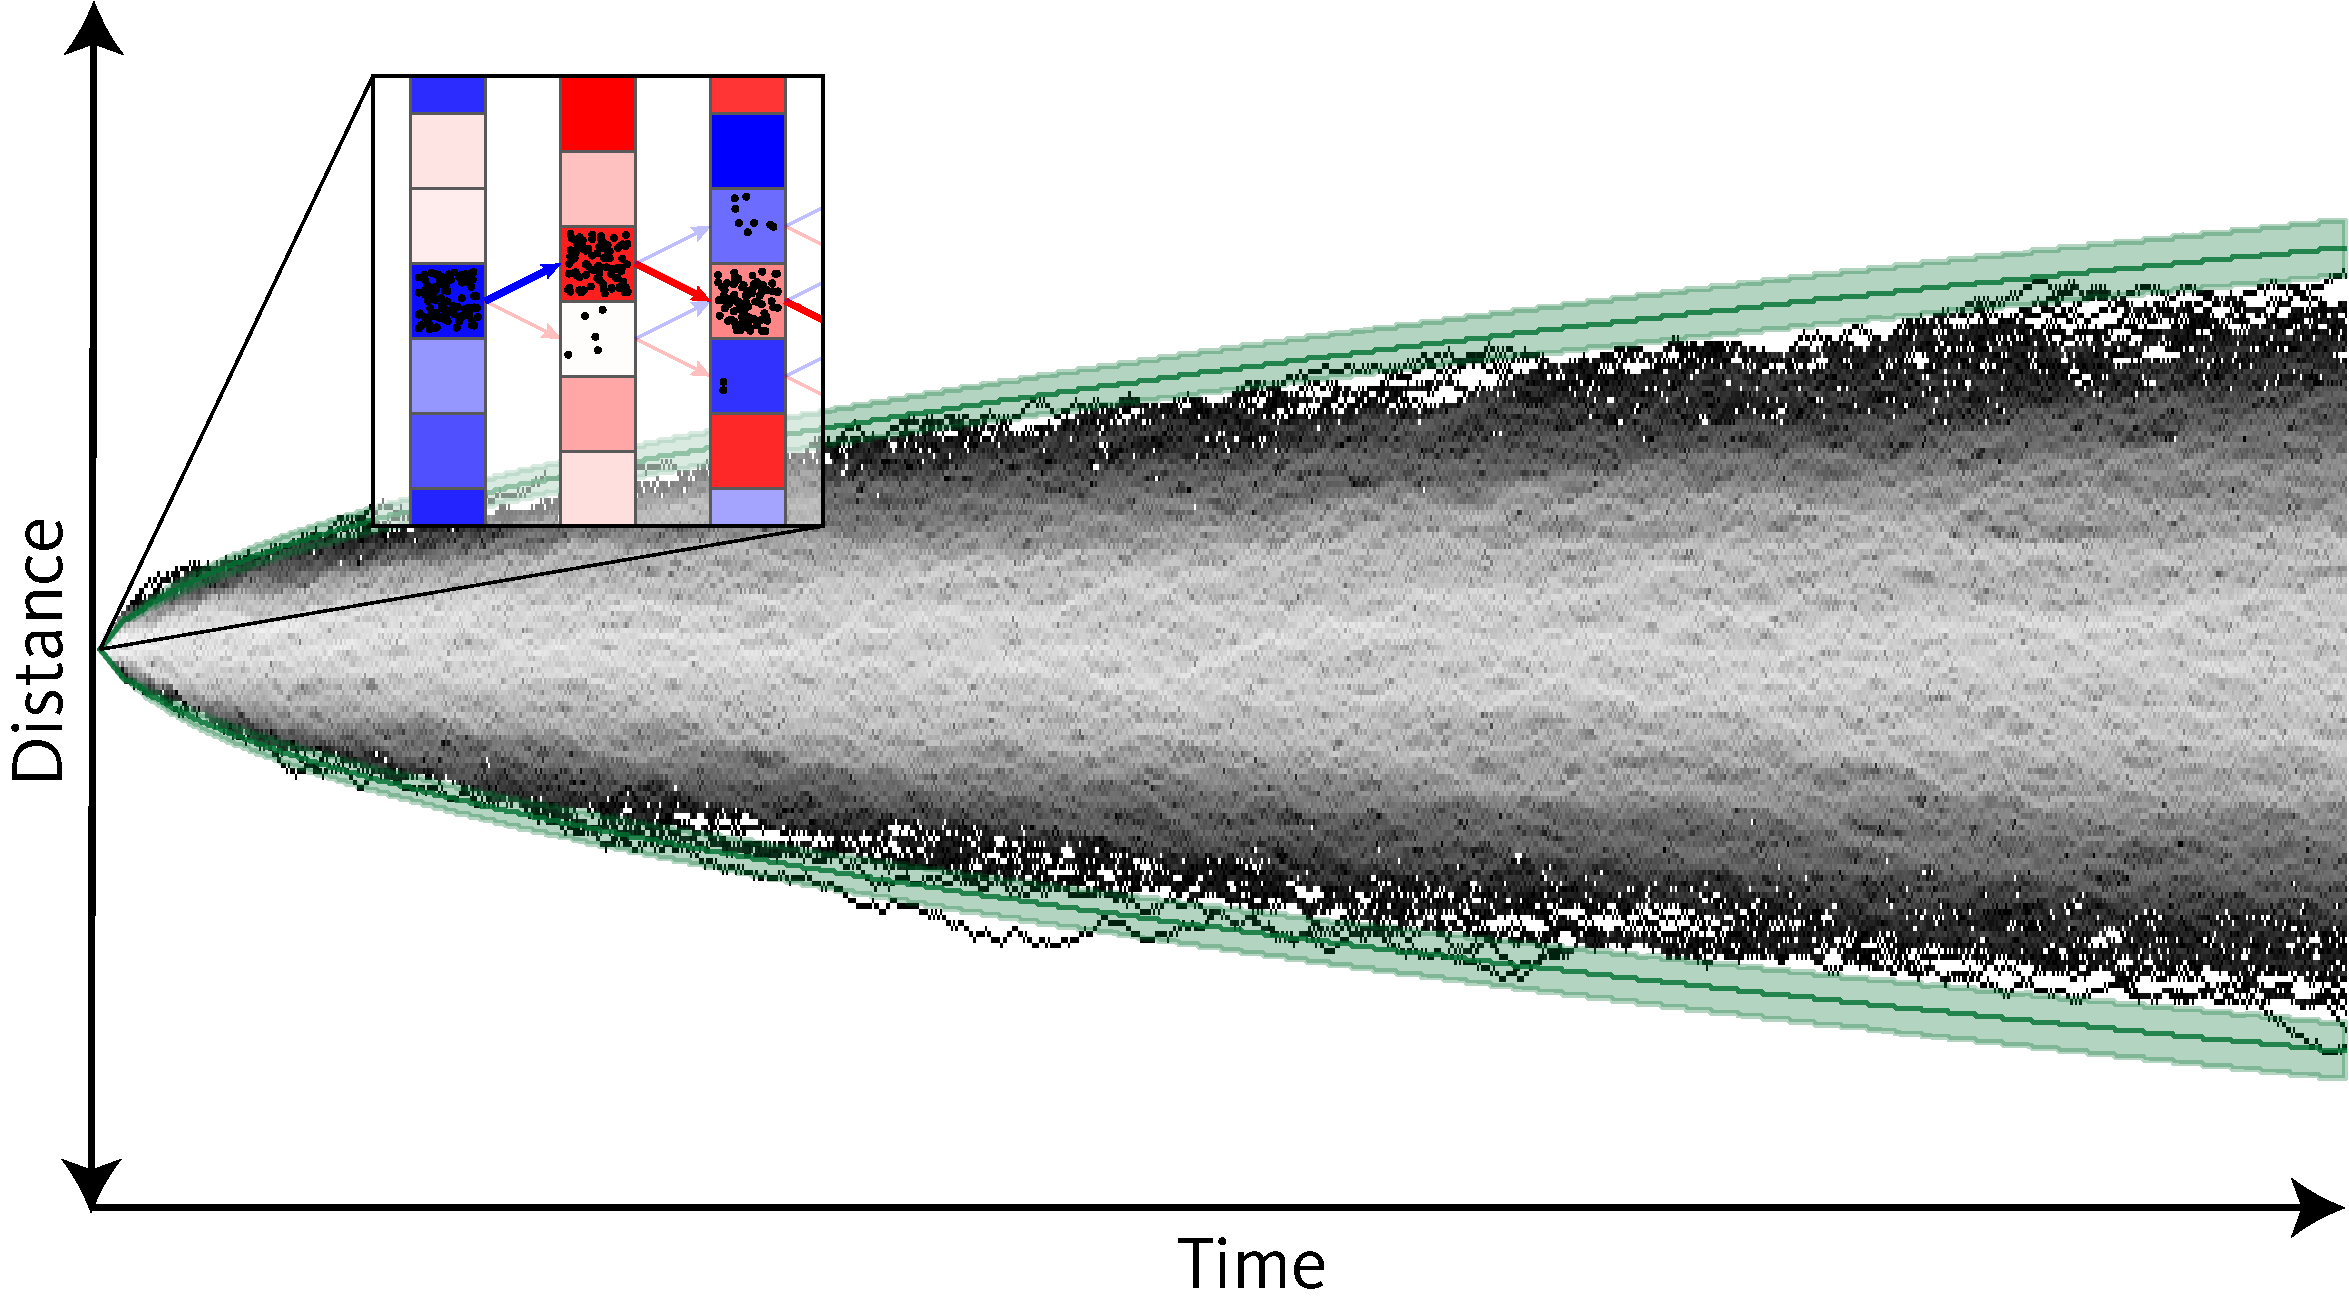
\includegraphics[width=.9\columnwidth]{Figures/Figure1.pdf}
  \caption{A system of $N=10^5$ particles evolving in a given random environment. The heat map records the site occupancy density. We also plot in green the asymptotic theory mean location for the maximum particle location. Around this is a shaded region with a width of two standard deviations based on the asymptotic theory variance. This region generally contains the extreme-most particle over time. The zoomed-in inset shows the spatial locations of $N=10^2$ particles over time. Color indicates the bias (red is biased down and blue is biased up) and is chosen independently at each space-time box. The location of particles within each box is chosen for ease of visualization.}
  \label{fig:BCModel}
\end{figure}

\section{Background}
Building on observations by Brown~\cite{brownXXVIIBriefAccount1828a, brownXXIVAdditionalRemarks1829a} from 1827,  Einstein~\cite{einsteinUberMolekularkinetischenTheorie1905b,einsteinZurTheorieBrownschen1906a, einsteinTheoretischeBemerkungenUber1907a} (along with Langevin~\cite{langevinTheorieMouvementBrownien1908a}, Sutherland~\cite{sutherlandLIIViscosityGases1893,sutherlandLXXVDynamicalTheory1905} and Smoluchowski~\cite{vonsmoluchowskiZurKinetischenTheorie1906, vonsmoluchowskiNotizUiberBerechnung1915}) proposed a theory of diffusion based on modeling particles by independent random walks with variance controlled by a diffusion coefficient intrinsic to the particle/environment pair. Soon after, Perrin experimentally verified Einstein's statistical predictions \cite{perrinMouvementBrownienRealite1909a, perrinMouvementBrownienMolecules1910a}.

Probing the effectiveness and limitations of Einstein's diffusion model has remained a challenge. On short time scales, particle motion is ballistic, dominated by inertia~\cite{uhlenbeckTheoryBrownianMotion1930a,huangDirectObservationFull2011,hammondDirectMeasurementBallistic2017,lukicDirectObservationNondiffusive2005, franoschResonancesArisingHydrodynamic2011, kheifetsObservationBrownianMotion2014}.
Many physically relevant situations require the addition of new concepts to accurately model them.
Certain diffusive processes are better modeled by Levy flights \cite{wangWhenBrownianDiffusion2012a} or other types of anomalous diffusions~\cite{bouchaudAnomalousDiffusionDisordered1990a, metzlerBrownianMotionFirstpassage2019a} instead of simple random walks. Other work has focused on active particles which inject energy into their environment~\cite{ramaswamyMechanicsStatisticsActive2010b,kanazawaLoopyLevyFlights2020a}. Further, in environments which are slowly mixing, Einstein's theory may also break down due to the presence of quenched disorder \cite{zangiFrequencydependentStokesEinsteinRelation2007, wangWhenBrownianDiffusion2012a}. Unlike the above deviations from the classical model, our approach is intended to describe generic many-particle diffusions.

The random walk in random environment (RWRE) model goes back to~\cite{chernovReplicationMulticomponentChain1967, temkinOnedimensionalRandomWalks1972} (see also~\cite{havlinDiffusionDisorderedMedia1987, bolthausenTenLecturesRandom2002,sznitmanTopicsRandomWalks2004, oferRandomWalksRandom2004, hughesRandomWalksRandom1995}) and comes in two types -- long-range~\cite{kestenLimitLawRandom1975,sinaiLimitingBehaviorOneDimensional1983a,bouchaudClassicalDiffusionParticle1990a, bouchaudAnomalousDiffusionDisordered1990a, burlatskyTransientRelaxationCharged1998, ledoussalRandomWalkersOnedimensional1999} and short-range~\cite{richardsonAtmosphericDiffusionShown1926, hentschelRelativeDiffusionTurbulent1984, bouchaudDiffusionLocalizationWaves1990,  chertkovAnomalousScalingExponents1996, bernardAnomalousScalingNPoint1996, jullienRichardsonPairDispersion1999a, balkovskyIntermittentDistributionInertial2001} temporally correlated environments. We focus here on the latter. In this context, typical RWRE particles behave like Brownian motion, matching the behavior from Einstein's model~\cite{rassoul-aghaAlmostSureInvariance2005, deuschelQuenchedInvariancePrinciple2016}.
The motion of atypical particles is controlled by large deviations of the RWRE's transition probability as first studied in ~\cite{balazsRandomAverageProcess2006}.

Barraquand and Corwin~\cite{barraquandRandomwalkBetadistributedRandom2017a} discovered the exactly solvable Beta RWRE discussed extensively below and uncovered a remarkable connection between its large deviations for times of order $\log(N)$ and the statistics of the Kardar-Parisi-Zhang (KPZ) universality class~\cite{corwinKardarParisiZhang2012a, quastelOneDimensionalKPZEquation2015a}, namely the Gaussian Unitary Ensemble (GUE) Tracy-Widom distribution~\cite{tracyLevelspacingDistributionsAiry1993}. Soon after~\cite{ledoussalDiffusionTimedependentRandom2017} recognized that a phase transition should occur in the $(\log(N))^2$ time frame while~\cite{barraquandModerateDeviationsDiffusion2020a} discovered that in this frame the GUE Tracy-Widom distribution is replaced by the KPZ equation one-point distribution~\cite{kardarDynamicScalingGrowing1986a,sasamotoOneDimensionalKardarParisiZhangEquation2010,calabreseFreeenergyDistributionDirected2010,dotsenkoBetheAnsatzDerivation2010,amirProbabilityDistributionFree2011}. See~\cite{sabotRandomWalksDirichlet2017,balazsLargeDeviationsWandering2019, barraquandLargeDeviationsSticky2020, barraquandLargeDeviationsSticky2020, brockingtonBetheAnsatzSticky2021, oviedoSecondOrderFluctuations2021,korotkikhHiddenDiagonalIntegrability2022,krajenbrinkCrossoverMacroscopicFluctuation2022} for further developments. The recursion relation \eqref{eq:kolmogorov} for RWRE transition probabilities solves a discrete version of the multiplicative noise stochastic heat equation (mSHE)
\begin{equation}
\partial_t Z(x,t) = \frac{1}{2} \partial_x^2 Z(x,t) + \xi(x,t)Z(x,t)
\end{equation}
with $\xi$ space-time white noise. The logarithm of the mSHE $h(x,t)=\log Z(x,t)$ solves the KPZ equation
\begin{equation}\label{eq:KPZ}
\partial_t h(x,t) = \frac{1}{2} \partial_x^2 h(x,t) + \frac{1}{2}(\partial_x h(x,t))^2 + \xi(x,t).
\end{equation}
Hence, large deviations for RWREs, in particular beyond the solvable model and even in experimental settings, may relate to the KPZ equation and its universality class -- especially in light of the rich canon of work on KPZ universality in various contexts using theoretical~\cite{albertsIntermediateDisorderRegime2010, corwinKardarParisiZhang2012a}, numerical~\cite{PhysRevA.45.638, prolhacHeightDistributionKPZ2011}, and experimental~\cite{halpin-healyKPZCocktailShakenNot2015a} methods. The KPZ connection is  quite useful since its statistics and power-laws are well studied.

\section{Models for diffusion}
Although physical diffusion is continuous in time and (typically) occurs in three-dimensional space, here we work with discrete models in one spatial dimension. The principal reason for this choice is that it is the setting for the exactly solvable  Beta RWRE~\cite{barraquandRandomwalkBetadistributedRandom2017a} (a continuous {\it sticky Brownian motion} limit of this model exists~\cite{barraquandLargeDeviationsSticky2020}) that will enable us to compare numerical results to exact theoretical predictions.
Beyond that, discretization is common for numerical simulations and higher dimensions are more challenging numerically due to anisotropy issues arising from the choice of lattice and due to the lack of exactly solvable models, c.f. \cite{ledoussalDiffusionTimedependentRandom2017}. In real diffusion in a common environment, there will be length and time scales on which the environment decorrelates.  Our discrete model can be thought of as coarse-graining the environment in space and time onto a lattice and thus we do not expect discrete and continuous models to differ greatly for long-times and large-scales. Our model ignores any higher order interactions as we expect them to be less present in the behavior of extreme particles, for which the local density is necessarily low. Additionally, there are physical settings where particles take discrete states~\cite{fellerDiffusionProcessesGenetics1951, moranRandomProcessesGenetics1958} or evolve in quasi-one-dimensional spaces~\cite{pollardGaseousSelfDiffusionLong1948,ahmadiDiffusionQuasionedimensionalChannels2017}.

We study the {\it Beta RWRE} introduced in~\cite{barraquandRandomwalkBetadistributedRandom2017a} (see Fig.~\ref{fig:BCModel}). We model the environment by a collection $\mathbf{B}= \big\{B(x,t):x\in \mathbb{Z},t\in \mathbb{Z}_{\geq 0}\big\}$ of independent identically distributed random variables all drawn from the uniform distribution on $[0,1]$. At time $t=0$ we start with $N$ particles all at site $0$. Given an instance of the environment $\mathbf{B}$ the particles proceed as follows. Each particle at $x$ and $t$ independently flips the same weighted coin which has probability $B(x,t)$ of heads (moving the particle to site $x+1$ at time $t+1$) and $1-B(x,t)$ of tails (moving to $x-1$ instead). Thus, while particles do not interact with each other, those at the same place and time are all influenced by the common environment.

This model is exactly solvable when $B(x,t)$ are distributed according to the Beta distribution, $Beta(\alpha, \beta)$~\cite{barraquandRandomwalkBetadistributedRandom2017a}. For simplicity, we focus on the special case $\alpha=\beta=1$ corresponding to the uniform distribution. The classical simple symmetric random walk (SSRW) model arises in the limit $\alpha=\beta\to \infty$ where all $B(x,t)\equiv 1/2$ and the environment is deterministic.

We focus on the behavior of the right-most particle at time $t$. We denote this by $\maxnt$, with $N$ the number of particles in the system. Two types of randomness affect $\maxnt$: that of the environment and that of sampling the random walks in that environment. The effect of the environment is via the transition probability $p_{\mathbf{B}}(x,t)$, the probability that a single random walker initially at $0$ will end up at $x$ at time $t$ for a given environment $\mathbf{B}$. This satisfies the recursion relationship, %(i.e., the Kolmogorov backward equation, or master equation),
%
\begin{align} \label{eq:kolmogorov}
 \begin{split}
  p_{\mathbf{B}}(x,t) = & p_{\mathbf{B}}(x-1,t-1)B(x-1,t-1) +\\
  & p_{\mathbf{B}}(x+1,t-1)\big(1-B(x+1,t-1)\big)
 \end{split}
\end{align}
%
with initial condition $p_{\mathbf{B}}(0,0) = 1$ and $p_{\mathbf{B}}(x \neq 0,0) = 0$. Since each random walker is independent, conditional on the environment, the distribution of the ensemble of $N$ walks is determined by $p_{\mathbf{B}}(x,t)$. Given the environment $\mathbf{B}$, the probability that a single random walker is at or above $x$ at time $t$ is given by the tail probability, $P_{\mathbf{B}}(x,t) = \sum_{y\geq x} p_{\mathbf{B}}(y,t)$. This and the independence of random walkers, conditional on the environment, imply
%
\begin{equation}\label{eq:maxpb}
\mathrm{Prob}_{\mathbf{B}}(\maxnt \leq x) = \big(1-P_{\mathbf{B}}(x,t)\big)^N,
\end{equation}
%
where the left-hand side is the probability, given the environment $\mathbf{B}$, that $\maxnt \leq x$.

We study how $\maxnt$ varies upon sampling a new environment and random walkers therein. Eq. \eqref{eq:maxpb} suggests that a good proxy for $\maxnt$ is the location $\envnt$ of the $1/N$-quantile of $P_{\mathbf{B}}(x,t)$, i.e., $\envnt$ equals the maximal $x$ such that $P_{\mathbf{B}}(x,t)>1/N$. Notice that $\envnt$ only accounts for the variation due to the environment. The variation due to sampling in that environment is denoted $\snt$ and defined by $\maxnt = \envnt + \snt$. We use the notation $\mean{\bullet}$ and $\var{\bullet}$ for the mean and variance of a quantity $\bullet$ (e.g. $\maxnt, \envnt,\snt$) averaged over both the environment and the sampling of random walkers in that environment.

\section{Numerical Methods}
We numerically simulate our models for system sizes varying from $N=10^2$ to $N=10^{300}$. We consider such large and physically unrealistic system sizes like $10^{300}$ in order to see how asymptotic theory applies for as wide a  range as possible of finite system sizes. We evolve the system for times from $t=0$ to $t= 5000 \log(N)$.  As explained below, $\log(N)$ and $(\log(N))^2$ set key timescales and our range of times ensure that for all choices of $N$, we encompass these scales. We simulate such large systems by tracking occupation variables instead of individual particle trajectories. In particular, if there are $N(x,t)$ particles at site $x$ at time $t$, then the number that move to site $x+1$ is binomially distributed with $N(x,t)$ samples and success probability $B(x,t)$ (the remainder move to site $x-1$). We sample these binomial distributions utilizing quadruple-precision floating point numbers and making approximations to the binomial distribution when dealing with sizes beyond our precision limits, as described in \cite{SeeSupplementalMaterial}. The rightmost particle location (identified by the maximal $x$ with $N(x,t)\geq 1$) at each time represents a sample of $\maxnt$. By repeatedly sampling new environments along with random walk occupation variables $N(x,t)$ therein we numerically measure $\var{\maxnt}$. To distinguish from the true value we denote this numerically measured variance by $\varnum{\maxnt}$ and plot it in Fig. \ref{fig:MaxVar}. In like fashion, we measure $\varnum{\envnt}$ for each sampled environment by using Eq. \ref{eq:kolmogorov} to compute $p_{\mathbf{B}}(x,t)$.  Fig. \ref{fig:QuantileVar} shows $\varnum{\envnt}$ as a function of time (see \cite{SeeSupplementalMaterial} for $\meannum{\maxnt}$ and $\meannum{\envnt}$). The data presented in Fig. \ref{fig:MaxVar} and \ref{fig:QuantileVar} took approximately three weeks to run in parallel on 500 cores of the University of Oregon high performance computing cluster, Talapas.

\begin{figure}[h]
 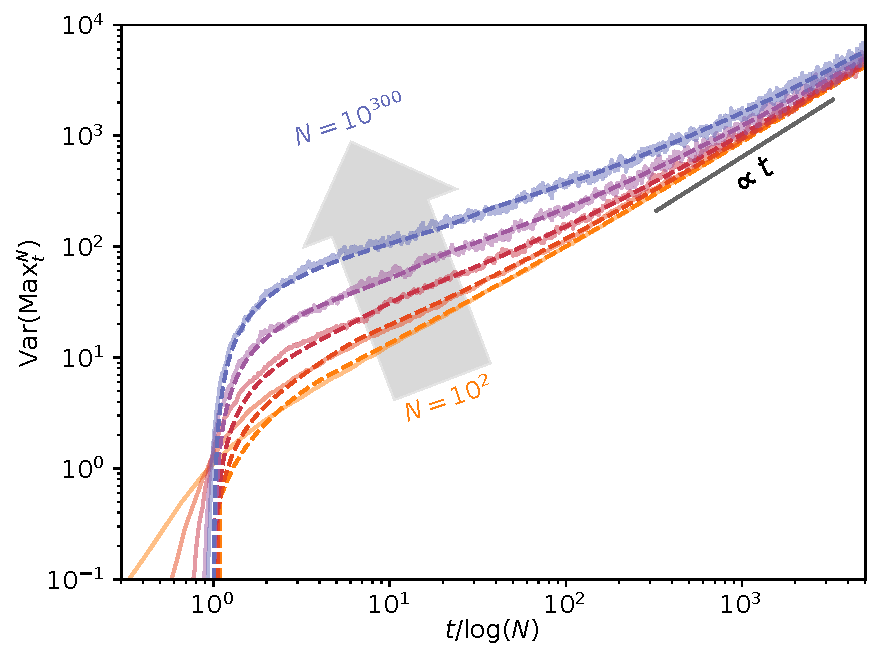
\includegraphics[width=\columnwidth]{Figures/MaxVar.pdf}
 \caption{Plots of $\varnum{\maxnt}$ (solid) computed over 10000, 5000, 1000, 500 and 500 environments (respectively) and  $\varasy{\maxnt}$ (dashed) for $N=10^2, 10^{7}, 10^{24}, 10^{85}, 10^{300}$}
 \label{fig:MaxVar}
\end{figure}

\begin{figure}[h]
	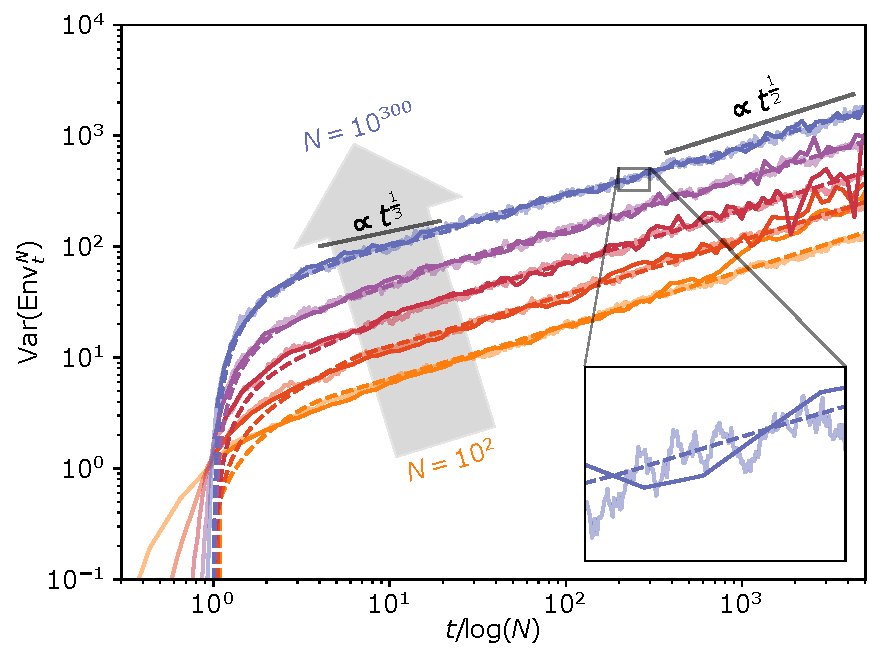
\includegraphics[width=\columnwidth]{Figures/QuantileVar.pdf}
	\caption{Plots of $\varnum{\envnt}$ (transparent solid) computed over 500 environments, $\varasy{\envnt}$ (dashed), and $\varnum{\maxnt} - \varasy{\snt}$ (dark solid) smoothed in each $1/25^{th}$ of a decade for $N=10^2, 10^{7}, 10^{24}, 10^{85},10^{300}$. The three curves agree as shown in the zoomed-in inset.}
	\label{fig:QuantileVar}
\end{figure}

\section{Asymptotic Theory Results}
We describe asymptotic results on the behavior of $\maxnt$, $\envnt$ and $\snt$ as both $N$ and $t$ tend to infinity in different limits. Given a fixed relationship between $t$ and $\log(N)$ such as $t/\log(N)=\hat{t}$ or  $t/\log(N)^2=\hathat{t}$ for $\hat{t}$ or $\hathat{t}$ fixed, we write $f(N,t)\gg g(N,t)$ if $f(N,t)/g(N,t)$ tends to infinity as $N$ and $t$ do subject to their relationship. We use the notation $\varasy{\bullet}$ to denote the asymptotic theory formula for the variance of $\bullet$, interpolated back to finite $N$ and $t$. SSRW theory follows from Stirling's formula while asymptotic results for the RWRE rely on tools from quantum integrable systems~\cite{barraquandRandomwalkBetadistributedRandom2017a, barraquandModerateDeviationsDiffusion2020a,krajenbrinkCrossoverMacroscopicFluctuation2022} and are derived first for $\envnt$ and then for $\maxnt$ and $\snt$.

\noindent\textbf{SSRW $\boldsymbol{\maxnt}$:}
For $t/\log(N)=\hat{t}$ with fixed $\hat{t} < (\log 2)^{-1}$, we have $N\gg 2^t$ and hence with very high probability every reachable site in the lattice at time $t$ is occupied, hence $\var{\maxnt}\approx 0$. When $\hat{t} > (\log 2)^{-1}$, we show  in \cite{SeeSupplementalMaterial} that $\maxnt$ is asymptotically a Gumbel random variable. For $\hat{t}$ large, $\varasy{\maxnt} \approx \frac{\pi^2}{12} \frac{t}{\log(N)}$.

%the location of the maximal random walk at time $t$ will likely occur at a position significantly below $t$ with non-trivial fluctuations which can be calculated by combining \eqref{eq:maxpb} with Stirling's formula for binomial coefficient asymptotics. Doing this in \cite{SeeSupplementalMaterial} we see that $\maxnt$ is asymptotically distributed as a Gumbel random variable. In particular, for $t\gg \log(N)$, $\varasy{\maxnt} \approx \frac{\pi^2}{12} \frac{t}{\log(N)}$.

\noindent\textbf{RWRE $\boldsymbol{\envnt}$:}
For $t/\log(N)=\hat{t}$ with fixed $\hat{t}<1$, $\var{\envnt}\approx 0$. To see this, note that $P_\mathbf{B}(t,t) = B_{0,0} \cdots B_{t-1,t-1}$. Taking logs and applying the central limit theorem shows that $\log \big(P_\mathbf{B}(t,t)\big) \approx -t  + t^{1/2} G$ for $G$ a standard Gaussian. This implies that $P_\mathbf{B}(t,t) \approx e^{-t}\gg 1/N$. Thus the RWRE stops saturating the lattice when $t= \log(N)$ plus a order $(\log(N))^{1/2}$ Gaussian fluctuation. For the SSRW this happens at time $\log_2(N)$ plus order one fluctuations.


$\var{\envnt}$ displays two asymptotic regimes. For fixed $t/\log(N)=\hat{t}>1$, $\var{\envnt}$ takes  asymptotic form,
\begin{equation}\label{eqlogN}
V_1(N, t):=\Big(\frac{\log(N)}{t}\Big)^{2/3} \sigma_{\chi}^2 \frac{2^{2/3}\big(1-\frac{\log(N)}{t}\big)^{4/3}}{1- \big(1- \frac{\log (N)}{t}\big)^2},
\end{equation}
where $\sigma_{\chi}^2\approx~0.813$ is the variance of the GUE Tracy-Widom distribution \cite{prahoferUniversalDistributionsGrowth2000, tracyLevelspacingDistributionsAiry1993}. As shown in \cite{SeeSupplementalMaterial}, this follows from the result of \cite{barraquandRandomwalkBetadistributedRandom2017a}: For $v\in(0,1)$, $\log P_\mathbf{B}(vt,t)=-t I(v) + t^{1/3} \sigma(v)\chi_t$ where $I(v) = 1-\sqrt{1-v^2}$, $\sigma(v) = (2I(v)^2/(1-I(v)))^{1/3}$ and $\chi_t$ is random converging to the GUE Tracy-Widom distribution as $t$ goes to infinity.

For $t/(\log(N))^2\!=\!\hathat{t}$,  $\var{\envnt}$ takes asymptotic form
\begin{equation}\label{eqlogNsq}
V_2(N, t):=\frac{t}{2\log(N)} \cdot \var{h\Big(0,\frac{4 (\log(N))^2}{t}\Big)},
\end{equation}
where $h(0,s)$ is the height at $0$ and time $s$ of the {\it narrow wedge} solution to the KPZ equation \eqref{eq:KPZ}. As shown in \cite{SeeSupplementalMaterial}, this follows from \cite{barraquandModerateDeviationsDiffusion2020a}: For $v\in (0,\infty)$,
$
\log P_\mathbf{B}(vt^{3/4},t) \approx -\frac{v^2t^{1/2}}{2} -\log(t)/4+\log(v) - v^4/12 + h(0,v^4).
$

Interpolating between these regimes, and extrapolating past $(\log(N))^2$ (see also \cite{krajenbrinkCrossoverMacroscopicFluctuation2022}) we find two power-laws,
\begin{equation}\label{eq:varqnt}
\varasy{\envnt} \approx
    \begin{cases}
    \sigma_{\chi}^2 (\frac{\log(N)}{2})^{\frac{1}{3}} t^{\frac{1}{3}}& 1 \ll \frac{t}{\log(N)}\ll \log(N),\\
    \frac{1}{2}\pi^{\frac{1}{2}} t^{\frac{1}{2}}& \frac{t}{\log(N)}\gg \log(N).
    \end{cases}
\end{equation}
For finite $N$ and $t$ these regimes have a gentle crossover that we capture by setting
$
\varasy{\envnt} := I(N,t) V_1(N, t)+\big(1-I(N,t)\big) V_2(N, t)
$
where $I(N,t) := \frac{1}{2} \cdot \left(1-\text{erf}\left(\frac{t-(\log(N))^{3/2}}{(\log(N))^{4/3}}\right)\right)$ (with  $\text{erf}(x)= 2/\sqrt{\pi} \int_{0}^{x} e^{-t^2}dt$ the error function) interpolates from $1$ to $0$ over an interval of width $(\log(N))^{4/3}$ around $(\log(N))^{3/2}$.


\noindent\textbf{RWRE $\boldsymbol{\snt}$ and $\boldsymbol{\maxnt}$:}
We identify the additional contribution from sampling the many-particle diffusion given an environment.
Using Eq. \eqref{eq:maxpb} and Taylor expansion of the results of \cite{barraquandRandomwalkBetadistributedRandom2017a} and \cite{barraquandModerateDeviationsDiffusion2020a} quoted above, \cite{SeeSupplementalMaterial} shows that for $t/\log(N)=\hat{t}>1$ the sample fluctuation $\snt$ is of Gumbel type with variance
%
\begin{equation}\label{eq:varnst}
\varasy{\snt} = \frac{\pi^2}{6} \frac{\big(\frac{t}{\log(N)} -1\big)^2}{2\frac{t}{\log(N)} -1}\approx \frac{\pi^2}{12} \frac{t}{\log(N)}
\end{equation}
as $\hat{t}$ grows. This limit matches the behavior of the SSRW model. In \cite{SeeSupplementalMaterial} we also show that $\snt$ is asymptotically independent of $\envnt$, thus
\begin{equation}\label{eq:varadd}
\var{\maxnt} \approx \var{\envnt} + \var{\snt}.
\end{equation}

\begin{figure}[h]
  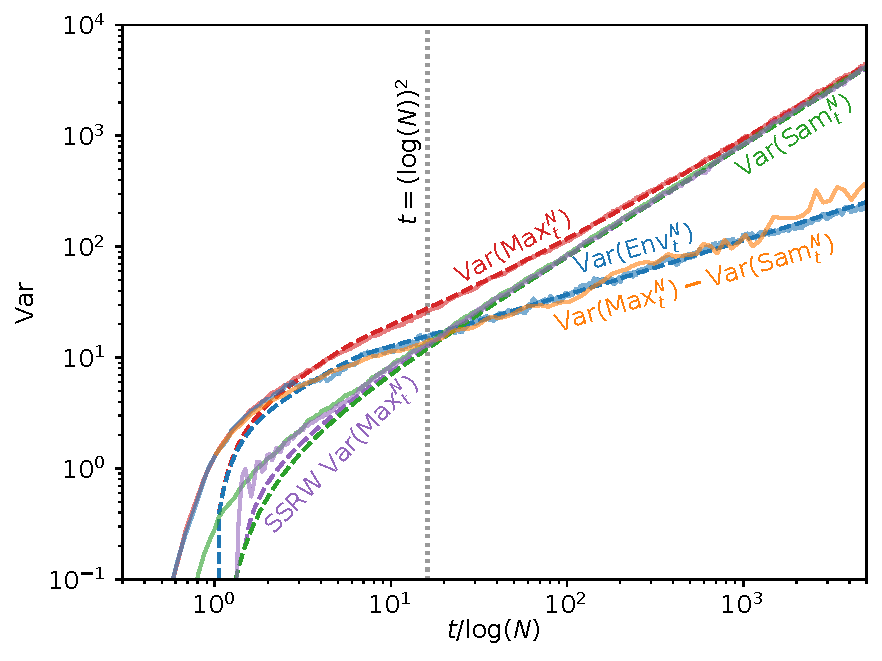
\includegraphics[width=\columnwidth]{Figures/MaxQuantComp.pdf}
  \caption{Variance of the maximal particle $\var{\maxnt}$ (red), environment $\var{\envnt}$ (blue), and sampling $\var{\snt}$ (green) for RWRE, and variance of the maximal particle  $\var{\maxnt}$ (purple) for SSRW, all for $N=10^7$. Dashed lines are $\varasy{\bullet}$, while solid lines are $\varnum{\bullet}$. $\varnum{\maxnt} - \varasy{\snt}$ (orange; smoothed as in Fig. \ref{fig:QuantileVar}) closely matches the environment curve (blue).}
  \label{fig:RWREAssembly}
\end{figure}

\section{Comparison of Numerical and Theoretical Results}
Fig. \ref{fig:MaxVar} and \ref{fig:QuantileVar} show that the asymptotic theoretical predictions for $\var{\maxnt}$ and $\var{\envnt}$ are in excellent agreement with the numerical measurements.  Fig. \ref{fig:QuantileVar} further shows that we reliably recover $\var{\envnt}$ using $\varnum{\maxnt} - \varasy{\snt}$, as expected from Eq. \ref{eq:varadd}. Notably, while these results were derived for asymptotically large $\log(N)$ and $t$, they hold nearly perfectly down to $N=10^{2}$.
Fig. \ref{fig:QuantileVar} reveals that while we readily see the long-time $t^{1/2}$ power-law for $\var{\envnt}$ from Eq. \ref{eq:varqnt}, the $t^{1/3}$ power-law is elusive. Although the full characterization of the short-time regime is in excellent agreement with the numerical results, the $t^{1/3}$ power-law is difficult to capture since the transitional window of $\log(N)$ to $(\log(N))^2$ is too narrow for realistic sizes of $N$, even up to $N=10^{300}$. By measuring the long-time $t^{1/2}$ power law, we measure the short-time scaling behavior of the KPZ equation up to a prefactor using Eq. \ref{eqlogNsq}. Fig. \ref{fig:RWREAssembly} shows the tight matching of the asymptotic theory curves and numerically measured values for the variance of $\maxnt, \envnt$ and $\snt$ for a given value of $N=10^7$. Notice that for $t\approx \log(N)$ the asymptotic theory and numerical values for the variance of $\snt$ do not fit as well as for large $t$. This is likely a result of finite-size effects and quickly goes away at larger values of $t$ or when $N$ increases. The fit for $N=10^{300}$ in Fig. \ref{fig:MaxVar} and \ref{fig:QuantileVar} remains tight over the entire range of $t$.

\section{Conclusion}
The link between RWREs and KPZ universality with its wealth of theoretical, numerical and experimental evidence strongly suggests that aspects of the picture presented here will persist beyond discrete and solvable models, even to experiments. When $t$ is of order $\log(N)$, variances should be non-universal, depending in a difficult to determine way on the nature of the environment. By contrast, when $t\gg\log(N)$, we anticipate that the scaling exponents and functional forms we have identified for the variances of $\envnt,\snt$ and $\maxnt$ will be universal, as will the relation \eqref{eq:varadd}. The leading coefficients  in Eq. \eqref{eq:varqnt} should be non-universal and hold within them all of the accessible information about the correlation structure of the environment -- we call these {\it extreme diffusion coefficients}. Further theoretical study, such as for the general $\alpha,\beta$ Beta RWRE model, should provide a natural first test of this universal picture and an understanding of how the extreme diffusion coefficients relate to the microscopic environment. A continuum model that should provide an even wider testing-ground amenable to numerics involves particles $x_i(t)$ for $i=1,2,\ldots$ satisfying $dx_i(t) = F(x_i(t),t)dt + D(x_i(t),t) dB_i(t)$ where $F(x,t)$ and $D(x,t)$ are random forcing (as in \cite{ledoussalDiffusionTimedependentRandom2017}) and diffusivity (generalizing diffusing diffusivity, c.f. \cite{PhysRevX.7.021002}) fields common to all particles while $B_i$ are  Brownian motions independent between different $i$. Changing the correlation structures of $F$ and $D$ will probe the transition between temporally mixing versus quenched environments, which should have very different behavior (c.f. \cite{PhysRevLett.61.500,PhysRevLett.62.3097}) and warrants further study. Considering higher dimensions as in~\cite{ledoussalDiffusionTimedependentRandom2017} may lead to further theory that better model real physical systems. A study of higher order cumulants may reveal other ways to probe the hidden environment, although they may be harder to observe numerically or experimentally.

In physical systems it is impossible to directly measure the environmental variance. However, an indirect measurement can be performed via the approach presented here by using $\var \envnt\approx \var \maxnt - \var \snt$. The sample variance $\var \snt$ is now computed using
$
 \var \snt = \frac{\pi^2 D}{6} \frac{t}{\log(N)}
$
where $D$ is the diffusion coefficient. One could repeatedly track the motion of the leading edge of diffusing particles in a system of colloids confined to a quasi-1D channel thereby directly measuring $\var \maxnt$ for system sizes ranging from $N ~ 10^2$ to $N ~ 10^{10}$. Further, one can also perform complementary measurements on the time of first passage of diffusing objects, which opens the door to experiments done on all manner of diffusing objects, including light or sound diffusing through a scattering medium, dye molecules in a fluid, or any other object whose first passage can be measured.
By measuring the environmental variance and extreme diffusion coefficient we will gain a new microscope through which to probe the hidden nature of the underlying environment in which the diffusion occurs. Our work should serve as a guide in the development and analysis of novel experimental measurements of the extreme behavior of many-particle diffusion.

\section{Acknowledgements}
We thank G. Barraquand and P. Le Doussal for discussions and S. Prolhac for providing numerics for $\var{h(0,s)}$.
This work was funded under the W.M. Keck Foundation Science and Engineering grant on ``Extreme Diffusion''.
I.C. also wishes to acknowledge ongoing support from the NSF through DMS:1811143 and DMS:1937254, the Simon Foundation through a Simons Fellowship in Mathematics (Grant No. 817655), and the Packard Foundation Fellowship for Science and Engineering. Much of this work was performed while I.C. held a Miller Visiting Professorship from the Miller Institute for Basic Research in Science, and while in residence at the Mathematical Sciences Research Institute in Berkeley, California (NSF Grant No. 1440140).
E.I.C. wishes to acknowledge ongoing support from the Simons Foundation for the collaboration Cracking the Glass Problem via award 454939. This work benefited from access to the University of Oregon high performance computing cluster, Talapas.


\section{Supplementary Material}
\label{ch2_supp}

\subsection{Numerical Methods}
\label{sec:Numerical}
We expand upon our description of the numerical methods used in our simulations. We consider varying system sizes from  $N=10^2$ to $N=10^{300}$ with time varying from $t=0$ to $t= 5000 \log(N)$. We simulate such large systems by utilizing the full range of quadruple-precision floating point numbers and making approximations to the binomial distribution when dealing with sizes beyond our precision limits. These approximations are necessary given the limitations of our precision and do not seem to affect the behavior of the system in any significant manner. In particular, for a site $x$ at time $t$ where the number of particles, $N(x,t)$, is below $2^{31}$ we use the C++ Boost integer implementation of a binomial distributed random number generator to choose the number of particles that will move right versus left. Above $2^{31}$ the integer implementation overflows and we instead  approximate the binomial distribution by a Gaussian distribution of mean $N(x,t) B(x,t)$ and variance $N(x,t)  B(x,t) (1 - B(x,t))$, as dictated by the central limit theorem. For sufficiently large $N(x,t)$, the variance itself will fall outside of the precision of a quadruple floating point number. This occurs when $N(x,t) > 10^{64}$, above which we approximate the binomial simply by its mean. The number of particles that move right is then $N(x,t) B(x,t)$. Psuodo-code of the simulation is given:

\begin{enumerate} 

 \item Start $N$ particles at $x=0$
 \item For each site:
  \subitem draw $B(x,t)$ from $\mathcal{U}_{[0, 1]}$
  \subitem if ($N(x, t) > 10^{64}$)
   \subsubitem $N(x+1, t+1) = N(x, t)B(x,t)$
   \subsubitem $N(x-1, t+1) = (1-B(x,t))N(x,t)$
  \subitem else if ($2^{31} < N(x, t) < 10^{64}$)
   \subsubitem $\mu = N(x,t)B(x,t)$
   \subsubitem $\sigma^2 = N(x,t)B(x,t)(1-B(x,t))$
   \subsubitem $N(x+1, t+1)$ is drawn from $\mathcal{N}(\mu, \sigma^2)$
   \subsubitem $N(x-1, t+1) = N(x, t) - N(x+1, t+1)$
  \subitem else if ($N(x, t) < 2^{31}$)
   \subsubitem $N(x+1, t+1)$ is drawn from $\mathrm{Bin}(N(x,t), B(x,t))$
   \subsubitem $N(x-1, t+1) = N(x,t) - N(x+1, t+1)$
\end{enumerate}

where $\mathcal{U}_{[0, 1]}$ is the random uniform distribution on the range $[0, 1]$, $\mathcal{N}(\mu, \sigma^2)$ is the Gaussian distribution with mean $\mu$ and variance $\sigma^2$, and $\mathrm{Bin}(n, p)$ is the Binomial distribution with number of trials $n$ and probability $p$. Note that our simulation differs from Monte Carlo, or agent based, simulations because we can group all the particles at a site together and iterate over each site. Our code is available at \url{https://github.com/CorwinLab/RWRE-Simulations}.

When estimating the statistics (e.g. mean and variance) for $\maxnt,\envnt$ and $\snt$, the optimal manner would be that for each $N$ and $t$ we simulate a large number of environments and then build up histograms for the behavior of these quantities with one data point corresponding to one environment. Of course, in numerically computing the quantities for time $t$, we naturally compute them for all times smaller than $t$ too, but for the same environment. Moreover, $\envnt$ can be computed simultaneously for all $N$ and $t$ relative to the same environment, providing even further computational savings. We employ this computationally efficient approach to couple together the estimation for different values of $N$ and $t$ to the same pool of environments. There is a cost, however, to doing this. For example, the statistics that we numerically compute for $\maxnt$ for time $t$ and time $t'$ will themselves be correlated since they are derived from studying the same collection of environments. This correlation seems to be short-lived in time though, and is only evident upon zooming into the numerical measurements, for instances as in the inset in Fig. \ref{fig:QuantileVar} of the main text.

\subsection{Asymptotic Theory Results}
\subsubsection{SSRW $\boldsymbol{\maxnt}$}\label{sec:SSRW}For the SSRW where $B(x,t)\equiv 1/2$, we use the same notation $p(x,t)$ and $P(x,t)$, dropping the $\mathbf{B}$ subscript. Now assume that the ratio $\hat{t} = t/\log(N)$ tends to some finite value. As explained in the main article, if $\hat{t}<(\log(2))^{-1}$ then $N\gg 2^t$. In that case, $p(t,t)=2^{-t} \gg 1/N$ which means that it is highly likely that there are many particles occupying the right-most site at $x=t$. This implies that $\mean{\maxnt}\approx t$ and $\var{\maxnt}\approx 0$.

When $\hat{t}> (\log(2))^{-1}$, the maximal random walk at time $t$ will likely occur significantly below $t$ and have non-trivial fluctuations which we now describe. For the SSRW, observe that $p(2k-t,t) =2^{-t} {t\choose k}$ for $k=0,\ldots, t$. Thus, using Stirling's formula for binomial coefficients (or more generally using Cramer's theorem from the large deviation theory for sums of independent identically distributed random variables) we arrive at the asymptotic for $v\in (0,1)$ that
\begin{equation}\label{eq:ldp}
P(vt,t) \approx e^{- t I_{\mathrm{SSRW}}(v)}\quad\textrm{where}\quad I_{\mathrm{SSRW}}(v) = \frac{1}{2}\big((1+v)\log(1+v) + (1-v)\log(1-v)\big).
\end{equation}
$I_{\mathrm{SSRW}}(v)$ is known of as the large deviation rate function for the SSRW.

We may now combine this with Eq. \eqref{eq:maxpb}  of the main text to show that
$\maxnt$ is approximately distributed as a Gumbel random variable with location
$\mu \approx t\hat v$ and shape  $\beta= 1/I_{\mathrm{SSRW}}^{\prime}(\hat v)$, where $\hat v=I_{\mathrm{SSRW}}^{-1}(1/\hat{t})$ (here $f^{-1}$ means the inverse function and not the reciprocal). A Gumbel random variable with location $\mu$ and shape $\beta$ has
\begin{equation}\label{eq:Gumbel}
\textrm{cumulative distribution function } e^{-e^{(-x-\mu)/\beta}},\quad \textrm{mean } \mu+\beta\gamma, \quad \textrm{and variance } \frac{\pi^2}{6}\beta^2,
\end{equation}
where $\gamma\sim .57721$ is the Euler-Mascheroni constant.


To see the above limit, observe that
\begin{align*}
&\mathrm{Prob}\big(\maxnt \leq t\hat{v}+x\big) = \big(1-P_{\mathbf{B}}(t\hat{v}+x,t)\big)^N \approx \big(1-  e^{- t I_{\mathrm{SSRW}}(\hat{v}+x/t)} \big)^N\\
&\approx \big(1-  e^{- t I_{\mathrm{SSRW}}(\hat{v}) - I'_{\mathrm{SSRW}}(\hat{v})x} \big)^N
=  \big(1-  N^{-1} e^{- I'_{\mathrm{SSRW}}(\hat{v})x} \big)^N \approx e^{-e^{- I'_{\mathrm{SSRW}}(\hat{v})x}}.
\end{align*}
The first equality follows from  Eq. \eqref{eq:maxpb}  of the main text, the second approximation uses \eqref{eq:ldp}, the third uses Taylor expansion, the fourth follows from the definition of $\hat v=I_{\mathrm{SSRW}}^{-1}(1/\hat{t})$, while the final one uses the approximation $(1-x/N)^{N}\approx e^{-x}$. Notice that in Taylor expanding we have assumed that lower order terms do not cause issues. This can be easily justified by going to further orders in the Stirling formula expansion.

Based on the above Gumbel asymptotics, we can now record the asymptotic form of the mean and variance of $\maxnt$ for the SSRW. Writing $\hat{v}(\hat{t})$ to make this dependence explicit and recalling that $\hat{t}= t/\log(N)$ we see that
\begin{equation}\label{eq:SSRWmeanvar}
\mean{\maxnt}\approx t\hat v\big(\tfrac{t}{\log(N)}\big) +  \frac{\gamma}{I_{\mathrm{SSRW}}^{\prime}\Big(\hat v\big(\frac{t}{\log(N)}\big)\Big)} ,\quad \var{\maxnt}\approx
 \frac{\pi^2}{ 6 \Big(I_{\mathrm{SSRW}}^{\prime}\Big(\hat v\big(\frac{t}{\log(N)}\big)\Big)\Big)^2}.
\end{equation}
Inverting $I_{\mathrm{SSRW}}$ to find $\hat v(\hat{t})$ is non-trivial though can be done numerically or in certain limits. For instance, noting that for $v$ near zero, $I_{\mathrm{SSRW}}\approx v^2/2$  we see that for $\hat{t}$ near infinity,  $\hat{v}(\hat{t})\approx \sqrt{2/\hat{t}}$ and hence
$I_{\mathrm{SSRW}}^{\prime}\big(\hat v(\hat{t})\big)\approx \sqrt{2/\hat{t}}$. From this and \eqref{eq:SSRWmeanvar} it follows that for $\hat{t}\gg  (\log(2))^{-1}$, asymptotically
$$
\mean{\maxnt}\approx \Big(\sqrt{2 \log(N)} + \frac{\gamma}{\sqrt{2 \log(N)}}\Big) t^{1/2},\qquad
\var{\maxnt}\approx \frac{\pi^2}{12}\frac{t}{\log(N)}.
$$
On the other hand, \eqref{eq:SSRWmeanvar} also shows that as $\hat{t}$ tends to $ (\log(2))^{-1}$ from above, the mean goes to $t$ and the variance goes to zero.

\subsubsection{RWRE $\envnt$}\label{sec:RWREenv}
Assume that the ratio $\hat{t} = t/\log(N)$ tends to some finite value exceeding $1$. The key theoretic result we use  here is due to \cite{barraquand_random-walk_2017}. They show that for $v\in (0,1)$,
%%
\begin{equation}\label{eq:bc}
\log\big(P_{\mathbf{B}}(vt,t)\big) = - t I(v)  + t^{1/3} \sigma(v)\chi_{t}\quad \textrm{where}\quad I(v) = 1- \sqrt{1- v^2},\quad\sigma(v) = \left(\frac{2 I(v)^2}{1-I(v)}\right)^{1/3}.
\end{equation}
Here $I(v)$ is the large deviation rate function and $\sigma(v) t^{1/3}$ is the scalings of the random environment-dependent fluctuations $\chi_t$ around that rate function. \cite{barraquand_random-walk_2017} showed that as $t\to\infty$, the distribution of $\chi_t$ converges to a Tracy-Widom GUE distribution $\chi$. For reference below, let us note that \cite{prahofer_universal_2000}
$$
\mu_\chi := \mean{\chi} \approx -1.771,\qquad \sigma_{\chi}^2 := \var{\chi}\approx .813.
$$

As in the case of the SSRW, we now solve for $\hat v=\hat v(\hat t)$ such that $P_{\mathbf{B}}(\hat vt,t)= 1/N$. Note that $\hat vt$ will then equal the $1/N$-quantile $\envnt$. From \eqref{eq:bc}, $\hat v$ must satisfy
\begin{equation}\label{eq:tIhat}
t I(\hat v) - t^{1/3} \sigma(\hat v) \chi_t =\log(N) = t/\hat{t}.
\end{equation}
Canceling $t$ and dropping the $t^{1/3}$ term momentarily yields to first order that $\hat v$ is given by
$$\hat v_0 = I^{-1}(1/\hat{t}) = \sqrt{1-(1-1/\hat{t})^2}.$$
We can now Taylor expand $I(\hat{v})$ and $\sigma(\hat v)$ in \eqref{eq:tIhat} around $\hat{v}=\hat{v}_0$ and solve for $\hat{v}$ to the next order. Doing so we find that
$$\hat{v} = \hat{v}_0 + t^{-2/3} \frac{\sigma(\hat{v}_0)}{I'(\hat{v}_0)} \chi_t + O(t^{-4/3}).$$
Recalling that $\hat{v} t$ is supposed to yield the $1/N$-quantile, we conclude that
\begin{equation}\label{eq:envntform}
\envnt = \hat v_0 t + t^{1/3} \frac{\sigma(\hat v_0)}{I'(\hat v_0)}  \chi_t + O(t^{-1/3}).
\end{equation}
From this we can extract the asymptotic mean and variance of $\envnt$. Written explicitly (i.e., plugging in $I$ and $\hat{v}_0$
) this yields the following asymptotic formulas
\begin{align*}
\mean{\envnt} &\approx M_1(N,t):= \Big(1-\big(1-\tfrac{\log(N)}{t}\big)^2\Big)^{1/2} t  +(\log(N))^{2/3} t^{-1/3}  \frac{2^{1/3} \big(1-\frac{\log(N)}{t}\big)^{2/3}}{\sqrt{1-\big(1-\frac{\log(N)}{t}\big)^2}} \mu_{\chi} \\
\var{\envnt}  &\approx V_1(N,t):= \Big(\frac{(\log(N))^{4/3}}{t^{2/3}}\Big)\frac{2^{2/3}\big(1-\frac{\log(N)}{t}\big)^{4/3}}{1- \big(1- \frac{\log (N)}{t}\big)^2} \sigma_{\chi}^2 ,
\end{align*}
where above we have used that
$$
\frac{\sigma(\hat{v}_0)}{I'(\hat{v}_0)}  = \frac{2^{1/3} \hat{t}^{-2/3} (1-1/\hat{t})^{2/3}}{\sqrt{1-(1-1/\hat{t})^2}}.
$$
For $\hat{t}=t/\log(N)$ large, it follows from the above expressions that
\begin{equation}\label{eq:varenvlogN}
\var{\envnt}  \approx  \sigma_{\chi}^2 \big(\tfrac{\log(N)}{2}\big)^{\frac{1}{3}} t^{\frac{1}{3}}.
\end{equation}
It is important to understand the order of the limits here. First we should fix $\hat{t}=t/\log(N)$ and take $N$ and $t$ to infinity. Then we take $\hat{t}$ large and find the above $1/3$ power-law. That said, with some additional work using the methods of  \cite{barraquand_random-walk_2017} it is possible to show that for the entire range $1\ll t/\log(N) \ll \log(N)$, this $1/3$ power-law persists. We will not provide the details for that here. However, below we will consider when $t$ is of order $(\log(N))^2$. In that case, for small $t$ in that range, we will find a perfect fit to the $1/3$ power-law, thus agreeing with the assertion that this power-law persists over the full range $1\ll t/\log(N) \ll \log(N)$.

\medskip
Now assume that the ratio $\hathat{t} = t/\log (N)^2$ remains strictly positive and finite as $N$ and $t$ tend to infinity.
While \cite{barraquand_random-walk_2017} probes $P_{\mathbf{B}}(x,t)$ for $x$ linearly growing with $t$, \cite{barraquand_moderate_2020} probes the regime where $x$ grows like $t^{3/4}$. They show that for $v\in (0,\infty)$,
\begin{equation}\label{eq:BLD}
\log\big(P_{\mathbf{B}}(v t^{3/4},t)\big)\approx  -\frac{v^2 t^{1/2}}{2} - \frac{\log(t)}{4} + \log(v) - \frac{v^4}{12}+ h(0,v^4)
\end{equation}
where $h(y,s)$ denotes the (random) height at spatial position $y$ and time $s$ of the {\it narrow wedge solution to the Kardar-Parisi-Zhang (KPZ) equation}
$$\partial_s h(y,s) = \tfrac{1}{2}\partial_y^2 h(y,s) + \tfrac{1}{2} \big(\partial_y h(y,s)\big)^2 +  \xi(y,s)$$
driven by space-time white noise $\xi$, see \cite{kardar_dynamic_1986, corwin_kardar_2012}. Using this result, we will be able to prove this other $(\log(N))^2$ time scale.

We may solve  \eqref{eq:BLD} perturbatively (as in the $\log(N)$ case) for $\hathat{v}$ such that $P_{\mathbf{B}}(\hathat{v}t^{3/4},t)= 1/N$. The $1/N$-quantile $\envnt=\hathat{v}t^{3/4}$ is then given by
$$
\envnt \approx \hathat{v}_0 t^{3/4} + \frac{t^{1/4}}{\hathat{v}_0}\left(h(0,\hathat{v}^4) - \frac{\hathat{v}_0^4}{12} -\log(\hathat{v}_0)\right) + O(t^{-1/4})\quad\textrm{where}\quad \hathat{v}_0 = 2^{1/2}\hathat{t}^{-1/4}.
$$
From this we can explicitly compute the asymptotics of the mean and variance as
\begin{align}\label{eq:var_longtime}
\nonumber \mean{\envnt} &\approx M_2(N,t):=  \big(2 t\log(N)\big)^{1/2} +\sqrt{\tfrac{t}{2\log(N)}}\mean{h\Big(0,\tfrac{4 (\log(N))^2}{t}\Big)}\\
\var{\envnt} &\approx V_2(N,t):= \tfrac{t}{2\log(N)} \cdot \var{h\Big(0,\tfrac{4 (\log(N))^2}{t}\Big)}.
\end{align}
Notice that in the mean we have dropped the lower order contributions from the terms $\frac{\hathat{v}_0^4}{12}$ and $\log(\hathat{v}_0)$.
The values of $\mean{h(0,s)}$ and $\var{h(0,s)}$ for varying $s>0$ can be computed numerically through evaluation of the Fredholm determinant formula from \cite{sasamoto_one-dimensional_2010,calabrese_free-energy_2010,dotsenko_bethe_2010,amir_probability_2011}.
The result of this computation is recorded as Fig. 3 of \cite{prolhac_height_2011}. In particular, the horizontal axis (labeled $t$ in  \cite{prolhac_height_2011}) corresponds to our $s$ variable, and the red circles record the value of $\mean{\frac{h(0,s)+\frac{s}{24}}{(s/2)^{1/3}}}$ while the blue triangles record the values of $\var{\frac{h(0,s)+\frac{s}{24}}{(s/2)^{1/3}}}$ (note that the $s/24$ shift here does not change the variance as it is deterministic). For $s>.33$ we approximate the mean and variances by interpolating between the numerically evaluated values in \cite{prolhac_height_2011} (S. Prolhac kindly provided the data set used to create Fig. 3 in that paper). For $s<.33$ we use the short-time behavior of the KPZ equation explained below for our values of the mean and variance.

There are two key asymptotics for $h(0,s)$ derived in \cite{sasamoto_one-dimensional_2010,calabrese_free-energy_2010,dotsenko_bethe_2010,amir_probability_2011}:
$\frac{h(0,s)+\frac{s}{24}}{(s/2)^{1/3}}\approx \chi$ as $s\to\infty$ where $\chi$ is a Tracy-Widom GUE distributed, and
$h(0,s)\approx -\tfrac{1}{2}\log(2\pi s) +s^{1/4} \pi^{1/4}2^{-1/2} G$ as $s\to 0$ where $G$ is standard Gaussian distributed.
These imply corresponding asymptotics for the mean and variance. In particular, as $\hathat{t}\to 0$,
$$
\var{\envnt} \approx \sigma_{\chi}^2 2^{-1/3} \log(N) \hathat{t}^{1/3}  = \sigma_{\chi}^2 \big(\tfrac{\log(N)}{2}\big)^{\frac{1}{3}} t^{\frac{1}{3}}
$$
which agrees perfectly  with \eqref{eq:varenvlogN}. This shows that the long-time behavior in the $t=O(\log(N))$ scaling regime and the short time behavior in the $t=O(\log (N)^2)$ scaling regime match even up to the pre-factor. This strongly suggests the $1/3$ power-law in Eq. \ref{I-eq:varqnt} of the main text for the entire regime $1 \ll t/\log(N) \ll \log (N)$.

On the other hand, from the short-time KPZ asymptotic we find that as $\hathat{t}\to \infty$,
$$
\var{\envnt} \approx \frac{1}{2} \pi^{1/2} t^{1/2}
$$
thereby recovering Eq. \eqref{eq:varqnt} for the regime $t\gg (\log(N))^2$ in the main text. This indicates that for finite $N$ and $t$ it is necessary to stitch together the two regimes to get a reasonable formula for $\var{\envnt}$.
We have found that an error function centered at $t=(\log(N))^{3/2}$ with a width of $(\log(N))^{4/3}$ produces a smooth transition between the two regimes. Thus, our final expression for the asymptotic mean and variance is given by
\begin{equation}
\label{eq:Var-Total}
\varasy{\envnt} = \frac{1-\text{erf}\left(\tfrac{t-(\log(N))^{3/2}}{(\log(N))^{4/3}}\right)}{2} V_1(N,t)+ \frac{1+\text{erf}\left(\tfrac{t-(\log(N))^{3/2}}{(\log(N))^{4/3}}\right)}{2}V_2(N,t),
\end{equation}
provided that $t\geq \log(N)$ and $0$ for $t<\log(N)$. Here $\text{erf}(x)= 2/\sqrt{\pi} \int_{0}^{x} e^{-t^2}dt$ is the error function. This construction is shown in Fig. \ref{fig:Interpolation}.
On the other hand, such stitching is unnecessary when it comes to the mean since the large $t$ behavior of $M_1(N,t)$ matches the behavior of $M_2(N,t)$ all the way as $t\to \infty$. This can be seen through direct asymptotics of the formulas and is illustrated in Fig. \ref{fig:MeanInterpolation}. On this account, we simply take
\begin{equation}
\label{eq:Mean-Total}
\meanasy{\envnt} =M_1(N,t).
\end{equation}

\begin{figure}[h]
\begin{center}
 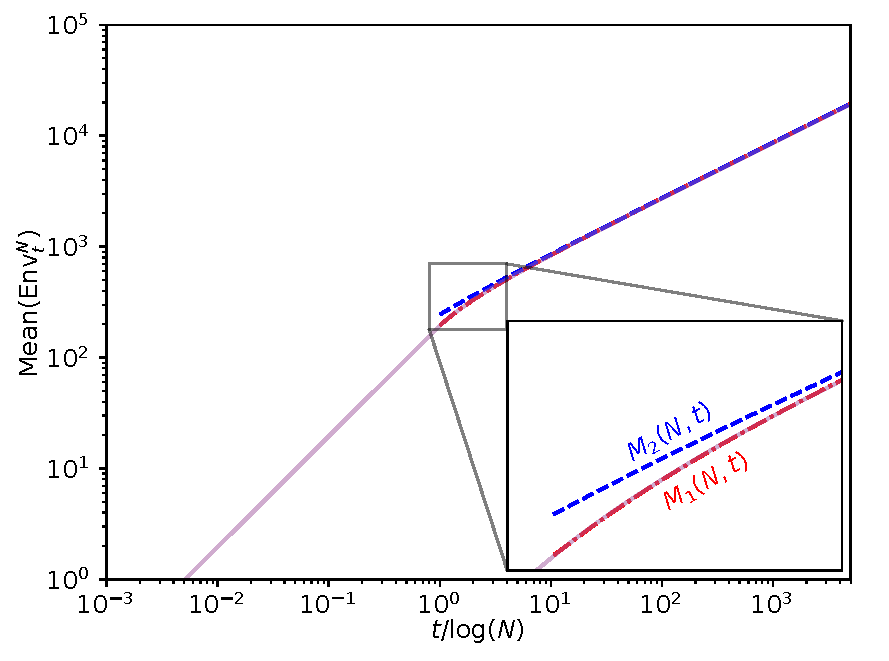
\includegraphics[width=0.8\columnwidth]{ch2_supplement/MeanInterpolation.pdf}
 \caption{The asymptotic mean functions $M_1(N,t)$ and $M_2(N,t)$ are plotted for $N=10^{85}$ in red and blue dashed lines, respectively. They agree closely for the full range of $t>\log(N)$ and also match the numerically measured values $\meannum{\maxnt}$ given by the purple curve (which is linear, as expected, until roughly time $t=\log(N)$).}
 \label{fig:MeanInterpolation}
\end{center}
\end{figure}

\begin{figure}[h]
\begin{center}
 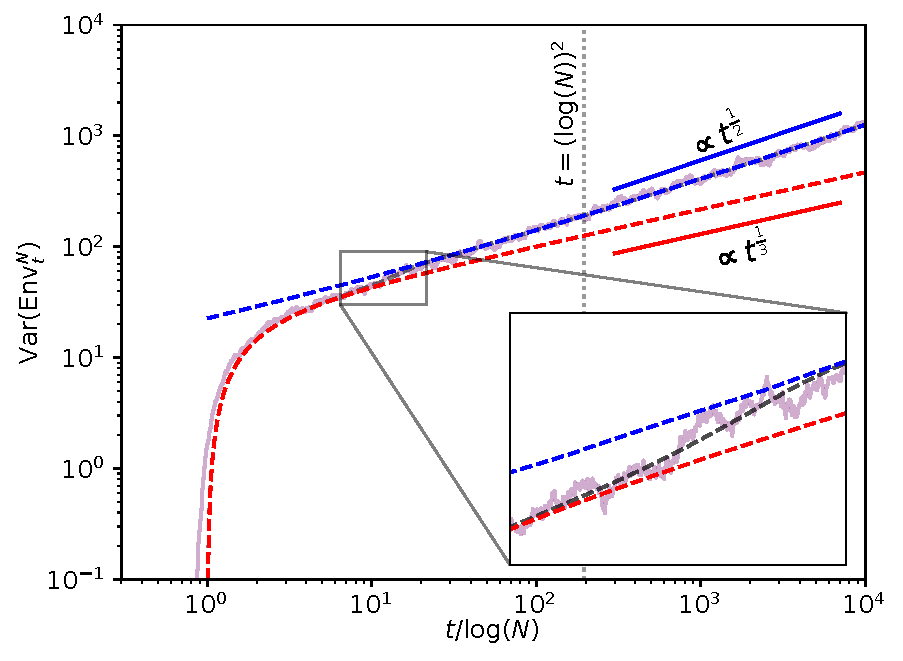
\includegraphics[width=0.8\columnwidth]{ch2_supplement/Interpolation.pdf}
 \caption{The asymptotic variance functions $V_1(N,t)$ and $V_2(N,t)$ are plotted for $N=10^{85}$ in red and blue dashed lines, and the stitched together formula for $\varasy{\envnt}$ from \eqref{eq:Var-Total} is plotted as the black dashed line. The purple curve is the numerically measured curve  $\varnum{\envnt}$. The inset shows how the stitching captures the transition between the two asymptotic curves $V_1$ and $V_2$, and the solid lines show the asymptotic power-laws that $V_1$ and $V_2$ demonstrate as $t\to\infty$. The vertical dotted line indicates the regime crossover at $t=(\log(N))^2$.}
 \label{fig:Interpolation}
\end{center}
\end{figure}

\subsubsection{RWRE $\snt$ and $\maxnt$}\label{sec:RWRE_Sam}
Assume for the moment that $t= \hat{t}\log(N)$ for $\hat{t}>1$. Then \eqref{eq:bc} implies that
$$
P_{\mathbf{B}}( \envnt + x,t) =\exp\Big(-tI\big(\tfrac{\envnt}{t} +\tfrac{x}{t}\big) + t^{1/3}\sigma\big(\tfrac{\envnt}{t} +\tfrac{x}{t}\big)\chi_t\Big)\qquad \textrm{and} \quad P_{\mathbf{B}}( \envnt,t) = \frac{1}{N}.
$$
If we Taylor expand to the next order in the exponential we find
\begin{align*}
P_{\mathbf{B}}( \envnt + x,t)&\approx \exp\Big(-tI\big(\tfrac{\envnt}{t}\big)-I'\big(\tfrac{\envnt}{t}\big)x + t^{1/3}\sigma\big(\tfrac{\envnt}{t}\big)\chi_t\Big)\\
&=\frac{1}{N} e^{-I'\big(\tfrac{\envnt}{t}\big)x} \approx\frac{1}{N}  e^{-I'(\hat{v}(\hat{t}))x}.
\end{align*}
The Taylor expansion requires a bit of explanation. We expand $I\big(\tfrac{\envnt}{t} +\tfrac{x}{t}\big) \approx I\big(\tfrac{\envnt}{t}\big) + I'\big(\tfrac{\envnt}{t}\big) \tfrac{x}{t}$ to first order. The similar expansion of $\sigma$ would produce a lower order term. However, there is a subtlety that we should point out. The $\chi_t$ random variable implicitly depends on $x$ as well. Namely, if we look at the random transition probability as we vary around $\envnt$, the fluctuations of this quantity will vary with $x$. However, we assume here that this fluctuation does not contribute to leading order. This assumption would be true if, for instance, $\chi_t$ looked locally like a random walk with independent and identically distributed intervals. This property is believed to be universal to models in the KPZ class and thus it is reasonable to assume that the same holds here. We do not attempt to justify this theoretically beyond this heuristic, though note that it yields very good agreement with our numerical simulations. The final approximation in the above string of equations involves replacing $I'\big(\tfrac{\envnt}{t}\big)x$ by $I'(\hat{v}(\hat{t}))x$ which relies on the fact that $\tfrac{\envnt}{t}\approx \hat{v}_0$ to highest order.

Combining the above deduction with \eqref{maxpb} in the main text and  $(1-x)^N\approx e^{-xN}$ (for $x$ small) yields
\begin{equation}\label{eq:SNT}
\mathrm{Prob}(\maxnt\leq \envnt + x) \approx \Big(1-\frac{1}{N}  e^{-I'(\hat{v}(\hat{t}))x}\Big)^{N}
\approx e^{-e^{-I'(\hat{v}(\hat{t}))x}}.
\end{equation}
If we define $\snt$ by the equality $\maxnt=\envnt+\snt$ then the above calculation shows that $\snt$ is asymptotically independent of $\envnt$ and asymptotically is Gumbel distributed with location and shape parameters
$$\mu(t)=0,\qquad \beta(t)=1/I'(\hat{v}(\hat{t})) = (\hat{t}-1)(2\hat{t}-1)^{-1/2}\approx (\hat t/2)^{1/2}$$
where the approximation is for $\hat{t}\gg 1$. This justifies the addition law for variances (Eq. \eqref{I-eq:varadd} in the main text)
\begin{equation}\label{eq:addlaw}
\var{\maxnt}\approx \var{\envnt}+\var{\snt}
\end{equation}
and (using the Gumbel variance formula in \eqref{eq:Gumbel}) this also justifies Eq. \eqref{I-eq:varnst} of the main text which provides the asymptotic formula for the variance (we also record that the asymptotic mean is 0)
\begin{equation}\label{eq:sntmeanvar}
\meanasy{\snt} =0,\qquad \varasy{\snt} = \frac{\pi^2}{6} \frac{\big(\frac{t}{\log(N)} -1\big)^2}{2\frac{t}{\log(N)} -1}\approx \frac{\pi^2}{12} \frac{t}{\log(N)},
\end{equation}
where the approximation is for $\hat{t}\gg 1$.

Putting together  \eqref{eq:Var-Total}, \eqref{eq:Mean-Total}, \eqref{eq:addlaw} and \eqref{eq:sntmeanvar} we conclude that
\begin{align}
\begin{split}
\label{eq:Var-Totalmaxnt}
\meanasy{\maxnt} &= M_1(N,t),\\
\varasy{\maxnt} &= \frac{1-\text{erf}\left(\tfrac{t-(\log(N))^{3/2}}{(\log(N))^{4/3}}\right)}{2} V_1(N,t)+ \frac{1+\text{erf}\left(\tfrac{t-(\log(N))^{3/2}}{(\log(N))^{4/3}}\right)}{2}V_2(N,t)\\&\quad+ \frac{\pi^2}{6} \frac{\big(\frac{t}{\log(N)} -1\big)^2}{2\frac{t}{\log(N)} -1}.
\end{split}
\end{align}

The above calculation assumed $\hat{t}=t/ \log(N)$ converges to a finite value. However, in a similar manner based on \eqref{eq:BLD} we can probe the behavior when $\hathat{t}= t/(\log(N))^2$ converges to a finite value. This behavior agrees perfectly with the large $\hat{t}$ limiting behavior above. Thus, we conclude that the formula for $\varasy{\snt}$ should hold for all $t\gg \log(N)$.

Fig. \ref{fig:MaxMean} show our asymptotic theory formulas for the mean of the maximal particle fit closely with our numerical simulations.


\begin{figure}[ht]
\begin{center}
 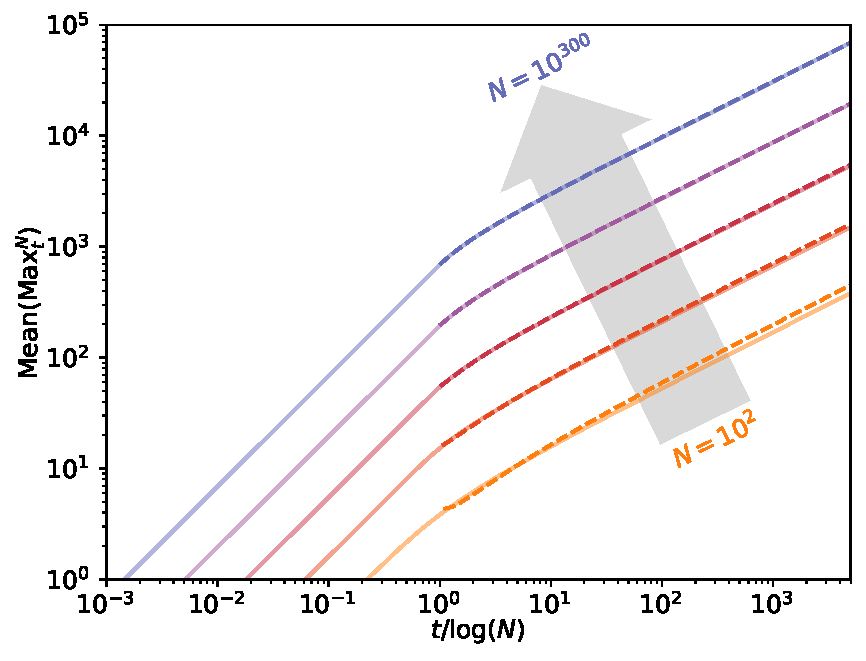
\includegraphics[width=0.8\columnwidth]{ch2_supplement/MaxMean.pdf}
 \caption{The mean position of the maximal particle location (solid line) for $N=10^2, 10^{7}, 10^{24}, 10^{85}$ and $10^{300}$ for $10000$, $5000$, $1000$, $500$ and $500$ instantiations of the environment, respectively. The theoretical prediction (dashed line) given in Eq. \eqref{eq:Var-Totalmaxnt} is also shown. We find the theoretical predictions for the mean position of the maximum particle, $\mean \maxnt$, are in agreement with the data.}
 \label{fig:MaxMean}
\end{center}
\end{figure}


\chapter{Colloid diffusion in glass capillary tubes}
\label{ch3_extras}

\section{Introduction}
Understanding the outliers in diffusive processes is the key to describing many important phenomena, such as biological processes dependent on the interactions between strands of DNA, patient zero spreading a virus to a new area in a pandemic, many chemical processes, and how microscopic price fluctuations relate to long-term macroscopic trends in the stock market~\cite{zhang_first-passage_2016, hufnagel_forecast_2004, redner_8_2001, liu_anchoring_2017}. How do we predict the behavior of these furthest or fastest particles? In diffusive environments, where many particles spread outward from their originating source, we can use Einstein’s treatment of diffusion to describe the bulk behavior of the particles~ \cite{einstein_uber_1905, von_smoluchowski_zur_1906}. Einstein described diffusion as particles undergoing independent random walks, but the independent nature of these walks ignores the effect the shared environment has on the particles. As a result, when analyzing the system as a whole, the distributions of outlier particle locations and first passage times should differ from those predicted by Einstein’s theory. We have designed an experimental system to measure the first passage times of micron-sized silica beads suspended in water travelling in narrow, quasi-1D glass capillary tubes to measure these extreme value statistics and demonstrate this difference.
 
% \begin{figure}[hb]
% \begin{center}
% 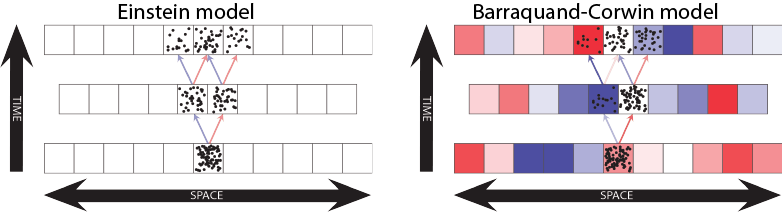
\includegraphics[width=0.9\columnwidth]{Figures/model_both_sidebyside.png}
% \caption{\label{fig:1D_BC} 1D visualization of the Einstein and Barraquand-Corwin models, where the red and blue colors indicate the direction of each bias - right and left, respectively - and the color intensity indicates the strength of the bias; for example, a dark red square indicates a strong bias to the right for the particles inhabiting that square. White squares have an equal bias in each direction. Time increases from the bottom of the image toward the top.}
% \end{center}
% \end{figure}

% \begin{figure*}[htp]
% \begin{center}
% 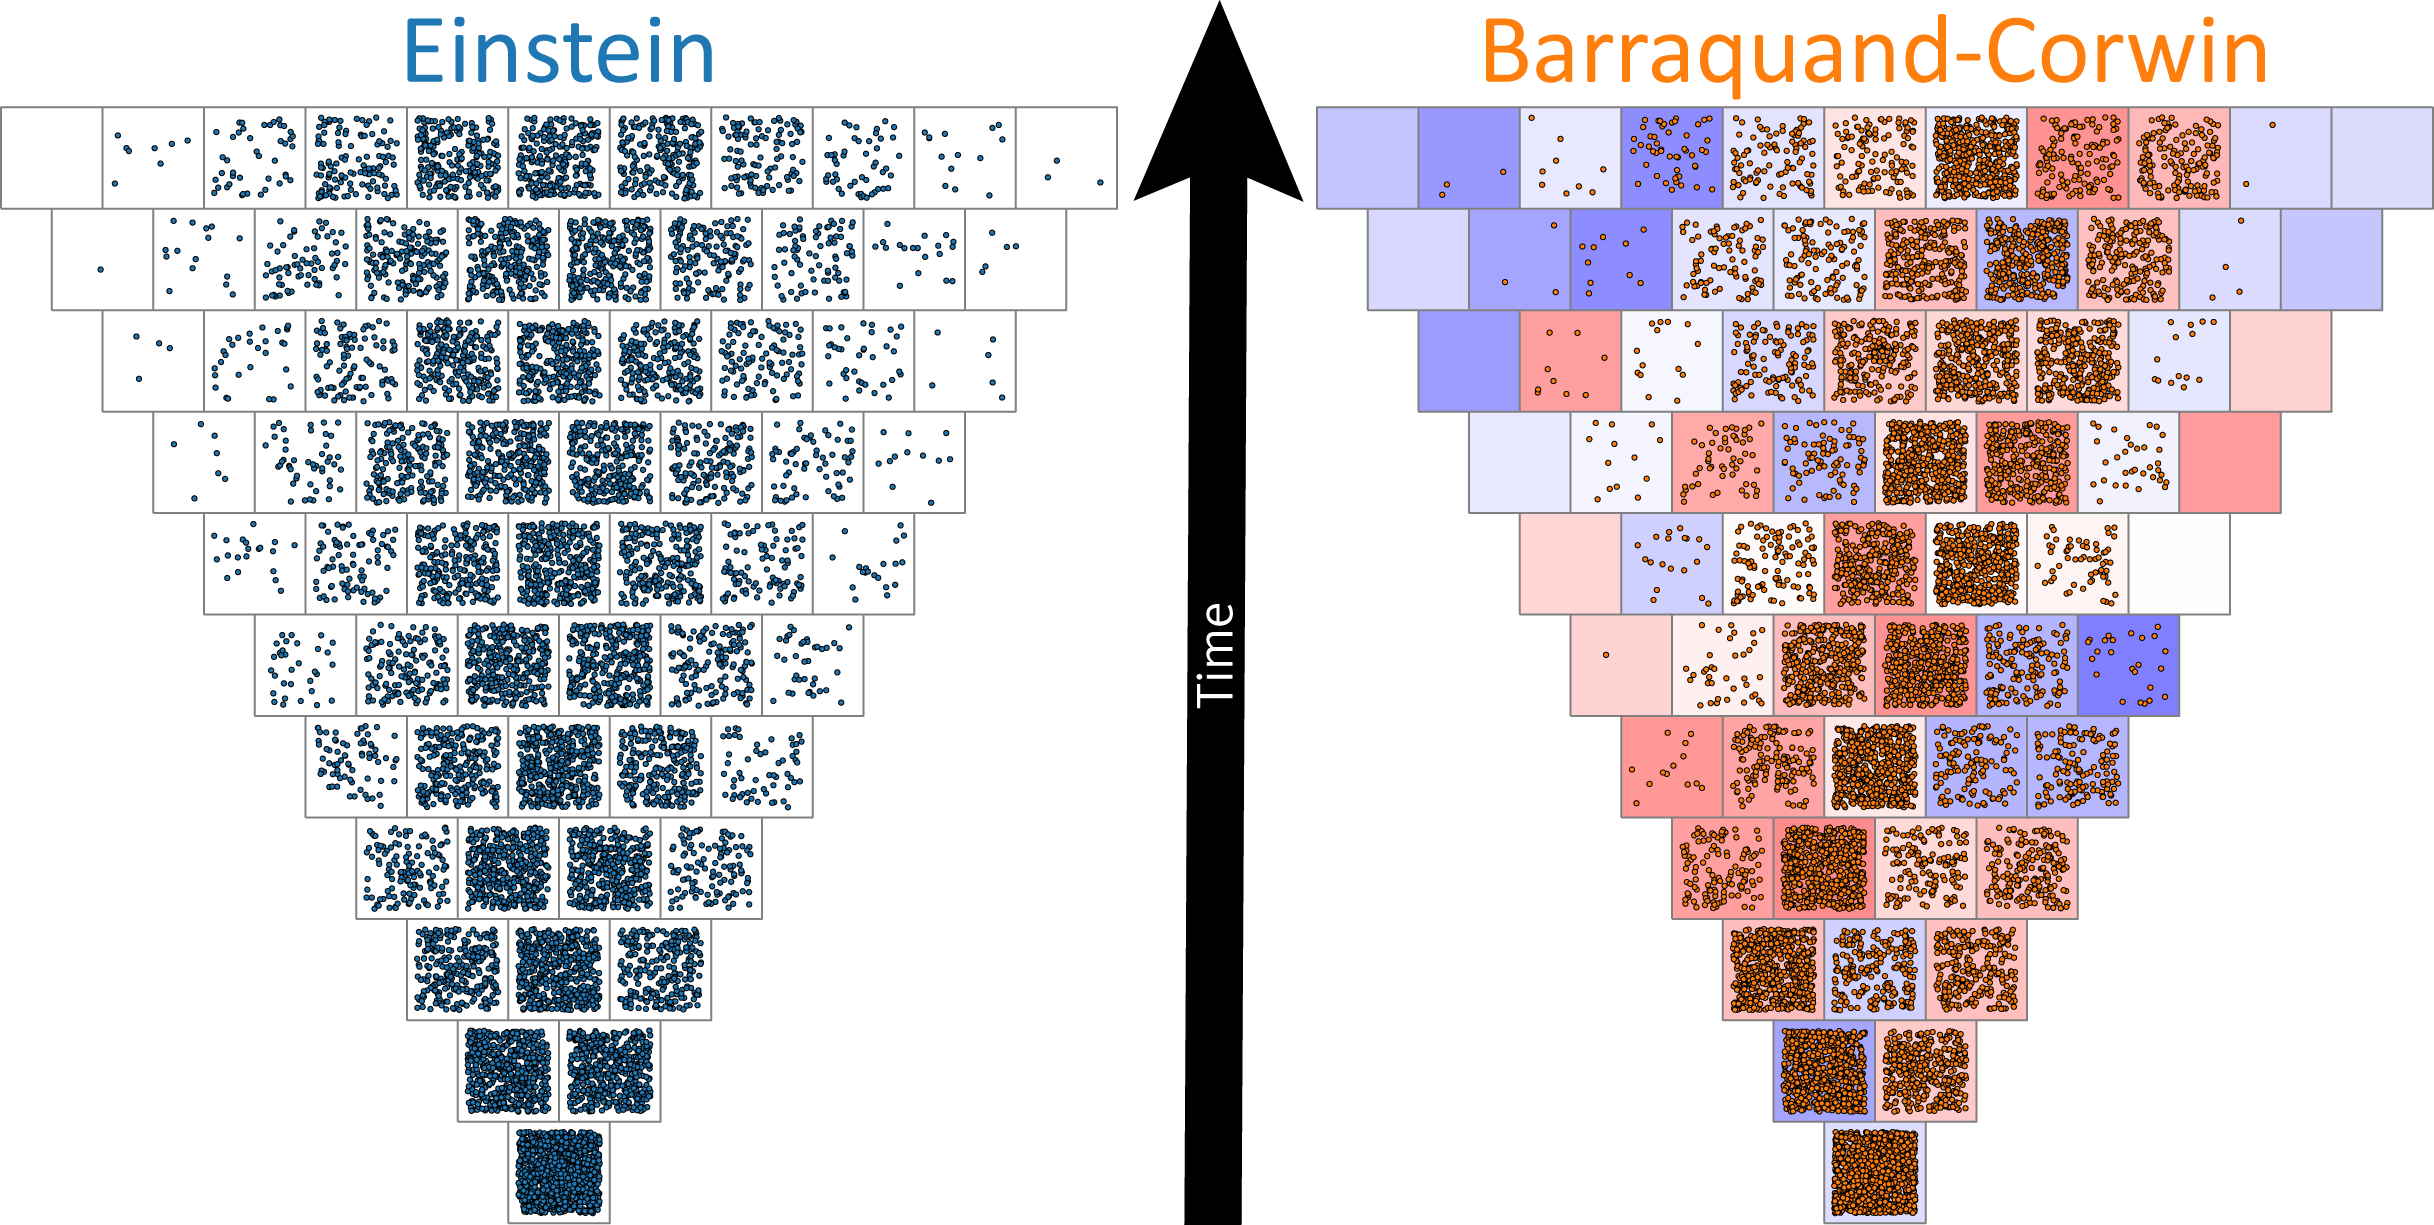
\includegraphics[width=0.9\columnwidth]{Figures/TriangleGrowth-01.png}
% \caption{\label{fig:comparison} Einstein and Barraquand-Corwin diffusion models. Einstein's diffusion model has an equal bias in each direction, and the particles diffuse accordingly. For the Barraquand-Corwin model, the red and blue colors and color intensity indicate the direction and strength of the bias as in Figure \ref{fig:1D_BC}. Time increases from the bottom of the image toward the top. There is a noticeable difference in how the outlier particles for each model spread in the same amount of time.}
% \end{center}
% \end{figure*}

\section{Background}
\acg{[determine how much of this is necessary given Chapter \ref{1Drandom}'s existence - this is mostly from comp exam and needs rewritten]}

While Einstein's traditional independent random walk model describes the average behavior well in many systems, there are areas where this theory and its predictions are known to fail. Some systems, such as Brownian motion in supercooled liquids and close to jamming, flow and drainage, friction, and turbulence, where probability distributions display exponential tails and other non-Gaussian characteristics~\cite{wang_when_2012, metzler_brownian_2019}. Additionally, Einstein’s theory fails to describe the full dynamics of active matter, where particles inject energy into the environment; such is the case with self-propelled particles exhibiting loopy trajectories and active particles capable of absorbing and dissipating energy~\cite{kanazawa_loopy_2020, ramaswamy_mechanics_2010}. The difference between systems with these dynamic particles and those well characterized by independent random walks is well described by contrasting these probability distributions, especially in the extremes.

\acg{[I need to revisit this claim] Studying and modelling first-passage particle behavior has been done, but this work often neglects systems where particle motion is correlated}~ \cite{grebenkov_exact_2020}. Guillaume Barraquand and Ivan Corwin developed a theoretical model for diffusion that explicitly includes correlations resulting from the shared background environment by modelling diffusion as a random walk with transition probabilities drawn from the beta distribution~ \cite{barraquand_random-walk_2017}. The Barraquand-Corwin model predicts the behavior of the maximum of a large number of ``walkers’’ and reveals a connection to the Kardar-Parisi-Zhang universality class with a related phase transition~ \cite{barraquand_random-walk_2017, barraquand_moderate_2020, le_doussal_diffusion_2017, kardar_dynamic_1986}. In times comparable to $log\left(N\right)$, there is a connection between the large deviations of transition probabilities in a random walk in random environment (RWRE) and the Kardar-Parisi-Zhang (KPZ) universality class's Tracy-Widom GUE distribution [cite lots of papers, see Hass paper]. In  the $log\left(N\right)^{2}$ time frame, the Tracy-Widom GUE distribution is replaced by that of the KPZ equation [also cite things from Hass paper, and Hass paper]. Numerical simulations from Chapter \ref{1Drandom} confirmed these scalings in these regimes.

Further work done by Hass et al\acg{[cite the FPT paper(s)]} describes how the first passage time scales with particle number.

%

\begin{figure*}[htp]
\begin{center}
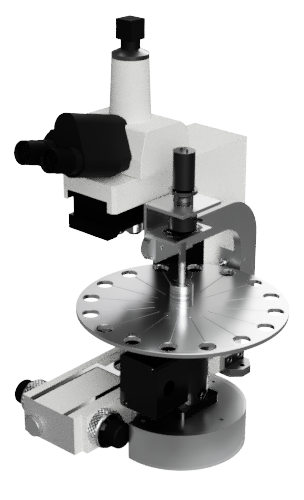
\includegraphics[width=0.35\columnwidth]{Figures/microscope_centrifuge.png}
\caption{\label{fig:CADrender} Experimental setup}
\end{center}
\end{figure*}

\acg{[first draft of everything below this point]}

\section{Experimental design}

To measure EFPTs in a physical system of colloids, we developed a microscope-centirfuge system, shown in Figure \ref{fig:CADrender}. The centrifuge consists of a flat rotor plate, which holds 16 samples and inside gaps for imaging, fixed to A DC motor (McMaster-Carr 59835K62) via screw-clamp bushing (McMaster-Carr 5926K16). Angular position of the plate is encoded by 16 bits via incremental optical rotary motion encoder (McMaster-Carr, 9749T2). By also tracking angular velocity via tachometer, we get down to 3mm positioning precision. A 12V sealed linear solenoid (McMaster-Carr 69905K173) acts as a brake to help lock in the final position. A custom machined aluminum base plate and support arm bolted to the optics table provide stability. A microcontroller (Arduino Mega) controls an external analog servo system, using a total of 19 digital pins -- 1 pin each to trigger the brake, turn servo mode on/off, and run the centrifuge at full speed outside of servo mode; in servo mode, 16 digital pins write a 16-bit location. The top speed of the centrifuge is currently unknown, but likely exceeds 1000 RPM. \acg{(mayhaps I should try to cover the holes and measure this again)}

An upright fixed stage microscope (Nikon ECLIPSE FN1) with either 4x or 10x objective (it is switchable, 4x gets more FOV but idk what it does about depth of field) with a camera (Teledyne Blackfly S USB3) is used to image silica microspheres (Cospheric monodisperse silica microspheres, 1.18 $\mu$m diameter) suspended in deionized (maybe bad?) water and sonicated to disperse aggregates, at a concentration of 1\% by volume. We coat the interior of 100mm long rectantular capillary tubes (Vitrocom VitroTubes™ 5003, 5004), 0.3mm/0.4mm wide and 0.03mm/0.04mm tall, with bovine serum albumin (BSA), flushing out the excess with pressurized air. This interior coating will help prevent silica microspheres from adhering to the capillary walls \acg{(cite someone that says this maybe?)}. We then fill the tubes with the silica suspensions, break off any air pockets, and seal the ends with capillary wax (Sigillum wax sealant). We dip the now-sealed ends in cyanoacrylate glue to provide a strong seal for when the centrifuge spins the samples down at high angular acceleration. The capillary surface is then cleaned with isopropyl alcohol and lens paper.

This process is repeated for 16 capillary tubes, with each tube placed into its own channel on the centrifuge plate. Care is taken to ensure the capillaries are as level/flat as possible to prevent gravity-driven flow in the solutions. Melted paraffin wax is carefully poured onto the non-imaging parts of each capillary, which, once cooled, adheres the capillaries in place in the channel. Once all 16 capillaries have been adhered, the centrifuge process may begin.

A MATLAB script controls both the Arduino for centrifuge operation and the camera for imaging. Upon starting the script, the Arduino pins and camera are initialized, and directories based on the datetime are created for data storage. The centrifuge enters run mode for a preset amount of time, where it spins at the highest attainable speed. After the time runs out, the centrifuge slows down, and the 16 position pins send it to the "16th" capillary location. The centrifuge then carefully pans through each location, collecting an initial "reference" image of each of the 16 capillaries. The script then enters time-lapse mode, where, based on a preset time gap, the centrifuge pans through each location and collects a new frame for each capillary. Each frame is stabilized relative to its initial "reference" frame and writing this corrected frame to an image file that capillary's image directory. After cycling through each capillary, the system pauses for the allotted time, then cycles through to collect and stabilize frames again. This repeats indefinitely, or until the user ends this sequence. The final parts of the script close the camera and clear all variables for the next collection.
 
\begin{figure*}[htp]
\begin{center}
\includegraphics[width=0.9\columnwidth]{Figures/capillaries.png}
\caption{\label{fig:caps} Examples of imaged capillaries}
\end{center}
\end{figure*}

\section{Results}
Preliminary results show that it is possible to centrifuge down samples in capillary tubes such that the majority of the colloids end up on the outer end. By removing air bubbles beforehand, and coating the tubes with bovine serum albumin, we minimize bulk flow and colloids sticking to the glass. Image stabilization removes discrepancies in the servo positioning and enables tracking of particles using packages such as Trackpy. Blah blah Figure \ref{fig:caps} shows issues. Would be nice to run tracking on sequence but idk if I'll get to that or not.

\section{Discussion/Conclusion}
While we have good descriptions for regular diffusion and average particles, and have been able to do so for a long time now, we have only recently been able to understand the extremes and characterize their statistical behavior. We have designed, built, and tested an experimental setup that allows us to measure first passage times in colloid diffusion. Further refinement is needed to make complete measurements, but preliminary results are promising, and the concept is sound.
%%

%\bibliography{scaling}% Produces the bibliography via BibTeX.


%\end{document}
%
% ****** End of file aipsamp.tex ******


\chapter{Measurements of extreme first passage times in photon transport}
\label{ch4_photons}

\section{Abstract}
Photon transport through turbid media has typically been modeled through diffusion or telegraph equations. These models describe behavior of the average, or typical, photon with remarkable accuracy, however, we show here that they fail to capture the Extreme First Passage Times (EFPTs) of photon transport. By sending ultra-fast bursts of photons through a scattering medium and timing the arrival of the first passage photon, we measure the distribution of these EFPTs of photons in a random environment. Our measured EFPTs differ from those predicted by both the diffusion approximation and telegraph equation. Instead, we observe the EFPT as the time expected for light to travel through an index-averaged medium. These results reveal flaws in both models and invite a re-examining of their underlying assumptions.

\section{Introduction}
When light passes through a scattering medium, the spatial distribution of photons is smeared out by random scattering events, resulting in a corresponding broadening of the distribution of photons from a pulsed source. This broadening has historically been modeled at short times by the telegraph equation~\cite{goldstein_diffusion_1951,ishimaru_diffusion_1989,durian_photon_1997,lemieux_diffusing-light_1998} and at asymptotically long times by the diffusion approximation~\cite{haskell_boundary_1994,bohren_absorption_1983,ishimaru_wave_1997}.  However, these models both rely on a central assumption, that the scattering, and thus the path through the system, of each photon is independent and identically distributed.  Here, we probe the quality of these models by examining a measurement of the Extreme First Passage Time (EFPT), that is, the \textit{first} time of first arrival within a pulse of light.  We use a femtosecond laser to fire pulses of light through a tunable scattering medium and measure the EFPT with a Single Photon Avalanche Diode (SPAD).  We present experimental evidence that both of these models provide quantitatively and qualitatively wrong predictions for this measurement. 

In this Letter, we review the history of models for the first passage of photons, then describe an experimental setup to measure photon EFPT. We describe the diffusion approximation and telegraph equation approaches to modeling photon transport, and compare EFPT predictions from these models to experimental measurements. We demonstrate that both models fail to predict the EFPT.

\section{Background}

Two widely used approximations for modeling photon transport are the diffusion approximation and the telegraph equation. The diffusion approximation predicts the bulk or average behavior of light pulses in random media and offers valuable insights into various systems across a broad range of applications~\cite{haskell_boundary_1994,  chandrasekhar_stochastic_1943,chandrasekhar_radiative_1950,  brown_light_1975, allgaier_diffuse_2021, taitelbaum_diagnosis_1999, amendola_accuracy_2021}. However, the diffusion approximation fails to incorporate ballistic photons and the speed of light, making it unsuitable for short length and time scales, media with significant anisotropy or absorption, or environments with low scattering~\cite{ishimaru_wave_1997, yoo_time-resolved_1990, yoo_when_1990, durian_photon_1997, zhang_wave_2002, pierrat_photon_2006}. The telegraph equation overcomes many of these limitations by accounting for the finite speed of light in a medium and capturing wave-like effects at small distances, providing a more accurate description of the bulk or typical behavior of light pulses~\cite{goldstein_diffusion_1951, durian_two-stream_1996, durian_photon_1997, lemieux_diffusing-light_1998, masoliver_solutions_1992, masoliver_finite-velocity_1996, das_non-fickian_1998, polishchuk_photon-density_1997}. Discrepancies remain at distances near the source relative to the transport mean free path~\cite{durian_photon_1997, dudko_photon_2005, lemieux_diffusing-light_1998}, and the accuracy of the predicted speed of light depends on how the scattering path length and anisotropy are treated during the derivation~\cite{ heizler_asymptotic_2012, hoenders_telegraphers_2005, polishchuk_photon-density_1997}.

\begin{figure}[h]
\begin{center}
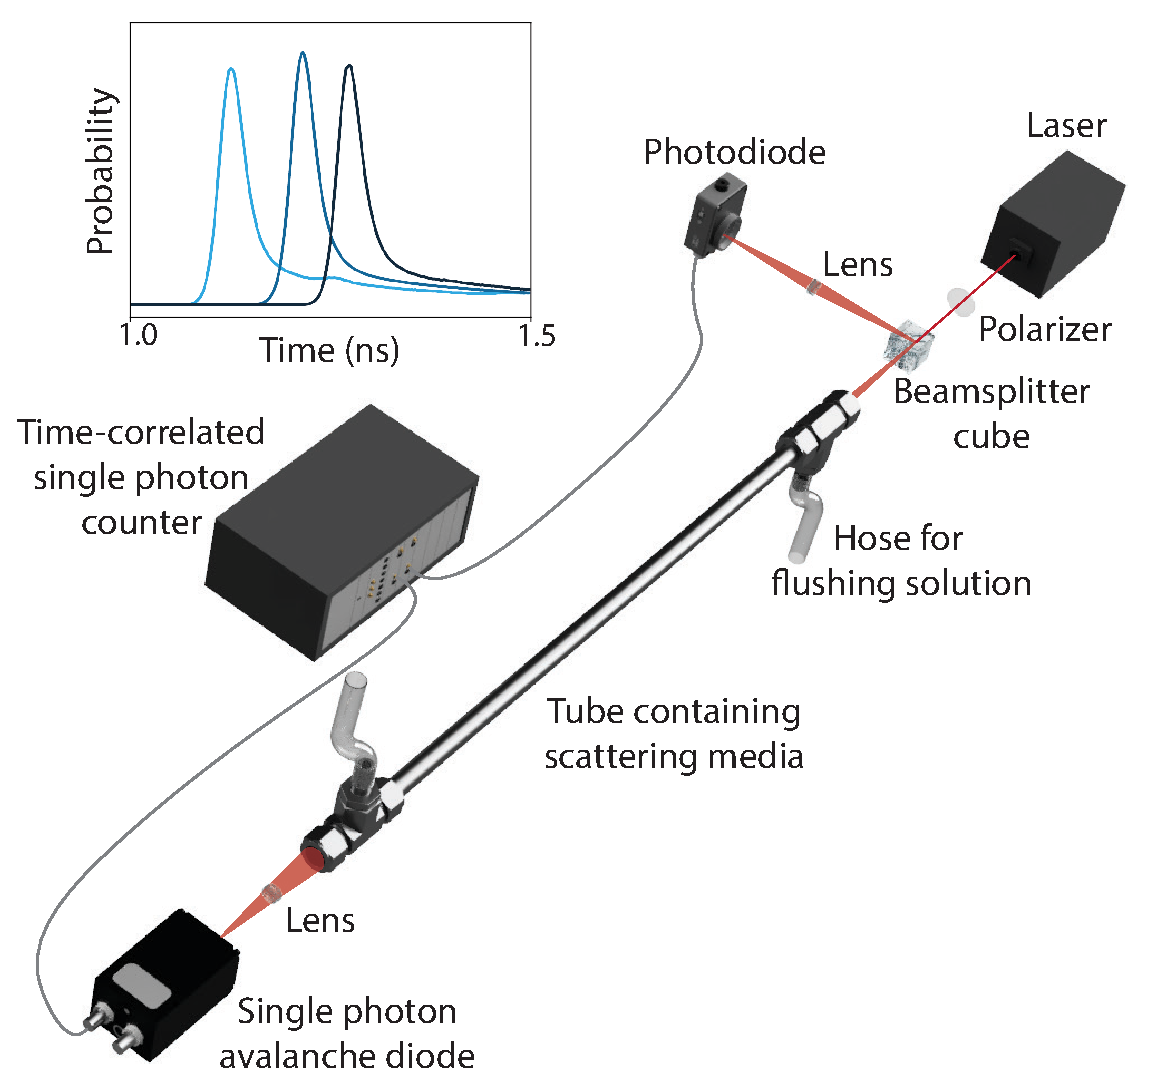
\includegraphics[width=0.8\columnwidth]{Figures/exp-setup-3.pdf}
\caption{\label{fig:setup}  Experimental setup, consisting of elements described in the text. Signals are collected over an adjustable time period, resulting in a histogram of EFPTs. An example of such a histogram at three different concentrations of scattering media is shown, with concentration increasing from left to right, where the x axis is the time relative to the speed of light in a vacuum, and the y axis is the probability of that time as the EFPT.}
\end{center}
\end{figure}

First passage times have been broadly described and studied across various diffusive systems~\cite{redner_guide_2001,weiss_applications_2002,godec_first_2016,noskowicz_average_1988}, including chemical and molecular reactions~\cite{redner_guide_2001,grebenkov_molecular_2021}, protein interactions~\cite{polizzi_mean_2016}, fractal media~\cite{chun_heterogeneous_2023}, and stock market fluctuations~\cite{barney_first-passage-time_2017,zsurkis_first_2024}. In general, extreme value distributions, which describe values drawn from the tails of a source distribution, exhibit distinct statistical behaviors~\cite{lawley_distribution_2020,lawley_universal_2020} and play a critical role in processes such as menopause timing~\cite{lawley_slowest_2023}, gene activation~\cite{schuss_redundancy_2019}, and oocyte fertilization by sperm~\cite{meerson_mortality_2015,schuss_redundancy_2019}.  In photonic systems, changes in pulse shape due to absorption and scattering have been measured~\cite{lee_using_2007,madsen_experimental_1992,ishimaru_diffusion_1978,yoo_time-resolved_1990,yoo_when_1990,zhang_wave_2002,calba_ultrashort_2008}, and photon first passage time distributions have been characterized numerically and experimentally~\cite{rossetto_isotropic_2022,long_particle_2001,weiss_applications_2002,zeller_light_2020}. To our knowledge, EFPT distributions have not previously been experimentally measured.


\section{Experimental Methods}\label{sec:exp_meth}
Our experimental setup is shown in Figure \ref{fig:setup}. Optical pulses of 140 fs in duration are generated with a femtosecond pulsed laser (Coherent Chameleon Ultra II laser) operating at central wavelengths tunable between 680-1080 nm with a repetition rate of 80 MHz and wavelength-dependent total output power range of 650-3500 mW. These pulses are sent through a power attenuating polarizer (Thorlabs GL10-B).  The majority of the power is bled off through a beamsplitter (Thorlabs BS041) and sent to a photodiode (Thorlabs DET10A).  This photodiode triggers a time-correlated single photon counter (TCSPC) (PicoQuant HydraHarp 400) to start a time-of-flight measurement.  The remainder of the light continues into a 12.7mm diameter, 1.015 m long stainless steel tube that has been internally polished.  This tube is filled with a solution of water and 20 nm diameter silica nanospheres (LUDOX AS-40). The nanospheres have an index of refraction $n$ = 1.453-1.456, dependent on wavelength.  The concentration of nanospheres is variable, in place, from volume fractions of 0 to 0.235 parts silica to 1 part water, where the maximum value is set by the volume fraction of undiluted LUDOX. The  concentration is adjusted by flushing the solution and flowing in a new solution.  After traveling through the scattering medium, photons exit the tube and are concentrated through a doublet lens (Thorlabs AC254-030-B-ML) onto a Single Photon Avalanche Diode (Micro Photon Devices PDM series SPAD).  The signal from the SPAD triggers the TCSPC to stop and the time of flight measurement is recorded. 

The TCSPC and SPAD both have a dead-time less than 80 ns, yielding an effective experimental repetition rate of 12.5 MHz. Using a detector for the TCSPC start and stop signals allows for measurement resolution that is not limited by the dead time. Integration times varied from 1-600 s.

The SPAD detection efficiency varies with wavelength from 10-30\%. From the peak laser power, approximately 3.5 W at 750 nm light, repetition rate of 80 MHz, and power attenuation from the optical components, we find a generous upper bound for the number of photons per pulse, $N$, entering the scattering medium as $5 \times 10^{6}$.

We use Ludox AS-40 as a scattering medium because it scatters strongly, absorbs minimally, is easily diluted with water, is slow to aggregate, and aggregation is easily reversed through sonication. Ludox has been well characterized for light scattering purposes~\cite{dezelic_determination_1960,bonnelycke_light_1959,goring_light-scattering_1957}. The small size of the silica nanospheres (roughly 3\% of the wavelengths used in these experiments) places us firmly within the Rayleigh scattering regime for which we can calculate $\sigma_{s}$ and $\mu_{s}$, the scattering cross section and coefficient, as~\cite{bohren_absorption_1983, chandrasekhar_radiative_1950} 
%
\begin{equation}\label{eq:scatter}
    \sigma_{s} =  \frac{2 \pi^{5}}{3} \frac{d^{6}}{\lambda^{4}}\left(\frac{n_{silica}^{2}-n_{water}^{2}}{n_{silica}^{2}+2n_{water}^{2}}\right)^{2},\ \mu_{s} = \frac{C}{\frac{4}{3} \pi \left(\frac{d}{2}\right)^{3}} \sigma_{s}
\end{equation}
%
where $d$ is the scatterer diameter, $\lambda$ is the wavelength of light being scattered, $n$ is the refractive index of the scatterer material, $C$ is the volume concentration of scatterers, and the scattering coefficient is the inverse of the scattering path length with units $\frac{1}{\textrm{m}}$. Using measurements performed with a UV/Vis/NIR spectrophotometer (Perkin Elmer Lambda-1050), we further characterize this medium by measuring $\sigma_{a}$, the absorption cross section, and use the Beer-Lambert law to find $\mu_{a}$, the absorption coefficient, as~\cite{lakowicz_principles_2006} 
%
\begin{equation}\label{eq:absorb}
    \sigma_{a} = 1.53\times 10^{-22}\ \textrm{m}^{2},\ \mu_{a} = \frac{C}{\frac{4}{3} \pi \left(\frac{d}{2}\right)^{3}} \sigma_{a}.
\end{equation}
%
% \acg{[NOTE: if useful to include, here lies the exact way to get from measured molar attenuation (in this case absorption) coefficient $\epsilon = 0.04$ to the absorption cross section $\sigma_{a}$}
% %
% \begin{equation}
%     \acg{\sigma_{a} = \ln{10} \frac{\rho_{water}}{N_{A}} \frac{\log_{10}\left(\frac{I_{0}}{I}\right)}{l C} }
% \end{equation}
% \acg{where $l$ is the path length of the cuvette, $C$ is the concentration of the solution, $I$ is the light intensity emitted, $I_{0}$ is the light intensity detected, $N_{A}$ is Avogadro's number, and $\rho_{water}$ is the density of water.}]
%

\section{Models for Photon Transport}\label{sec:predictions}
A classical approximation to the spatial and temporal distribution of photons is the equation of transfer ~\cite{haskell_boundary_1994,ishimaru_wave_1997}. As there is currently no general solution to  this time-dependent radiative transfer equation, most applications rely on approximations to derive a more tractable solution. Different approximation methods yield distinct solutions, with the diffusion approximation and the telegraph equation being two widely used approaches. In the following, we approximate the transmission of light through a slender tube filled with scattering medium as a one-dimensional process. We describe these two approaches below, resulting in two distinct photon probability distributions. From the probability distribution of photon locations, we derive an approximation for the extreme first passage time (EFPT) past a distance $L$. We approximate this as the first time at which the cumulative probability beyond $L$ surpasses 1/$N$, for $N$ incident photons~\cite{hass_first-passage_2024}.

\subsection{The equation of transfer}
The equation of transfer is given by ~\cite{haskell_boundary_1994,ishimaru_wave_1997},
%
\begin{align}
    \frac{1}{c} &\partial_{t} L \left(\mathbf{r},\hat{s},t\right) + \mathbf{\nabla} \cdot L\left(\mathbf{r},\hat{s},t\right)\hat{s} = -\left(\mu_{s} + \mu_{a}\right) L\left(\mathbf{r},\hat{s},t\right) \nonumber \\
    &+ \mu_{s} \int \int_{4\pi} L\left(\mathbf{r},\hat{s'},t\right) f\left(\hat{s} \cdot \hat s'\right) d\Omega' + S\left(\mathbf{r},\hat{s},t\right). \label{eq:RTE}
\end{align}
%
This equation determines the rate of change of the radiance, $L$, through position $\mathbf{r}$, in direction $\hat s$, and at time $t$. The radiance originates at a source, described by $S$, and is lost to the absorption coefficient, $\mu_{a}$, and scattered by the scattering coefficient, $\mu_{s}$. The speed of light in the medium is $c$, and $f(\hat s \cdot \hat s')$ is the normalized differential scattering probability for photons traveling in a direction $\hat s'$ to scatter into the direction $\hat s$. 

\eqref{eq:RTE} can be integrated over all solid angles to find a continuity equation governed by the photon density, $\varphi\left(\mathbf{r}, t\right)$, and photon flux, $\mathbf{j}\left(\mathbf{r}, t\right)$~\cite{haskell_boundary_1994}. When considering scattering in a long tube it is useful to approximate the system as quasi-one-dimensional.  Because $f\left(\hat{s}\cdot\hat{s}'\right)$ can be thought of as a distribution of scattering angles where $\cos \theta = \hat s \cdot \hat s'$, it will reduce to a single parameter, $\langle\cos{\theta}\rangle$, when integrated over all angles. For Rayleigh scattering, which is isotropic in both forward and backward directions~\cite{bohren_absorption_1983}, $\langle\cos{\theta}\rangle = 0$.

\subsection{Diffusion approximation}\label{sec:diffusion}
When the total volume concentration of scatterers greatly exceeds 1\%, \eqref{eq:RTE} can be estimated by a diffusion approximation. Under the assumption that photons interact with many particles, we assume a nearly uniform angular scattering distribution~\cite{ishimaru_wave_1997,bohren_absorption_1983}. By expressing the radiance $L\left(\mathbf{r},t\right)$ as the sum of an isotropic photon density $\varphi\left(\mathbf{r}, t\right)$ and a small directional flux, neglecting variations and anisotropy in the source term $S\left(\mathbf{r},t\right)$, integrating over all solid angles, and approximating as a one-dimensional system, we obtain~\cite{haskell_boundary_1994}
%
\begin{equation}\label{eq:diff}
    D \partial_{r}^{2} \varphi \left(r,t\right) - \mu_{a} c \varphi \left(r,t\right) = \partial_{t} \varphi \left(r,t\right) - c S \left(r,t\right),
\end{equation}
%
with diffusion coefficient
\begin{equation}\label{eq:diffD}
    D = \frac{c}{3\left(\mu_{s} + \mu_{a}\right)}.
\end{equation}
The solution to \eqref{eq:diff} is well-established as a Gaussian multiplied by a decaying exponential term that accounts for absorption~\cite{haskell_boundary_1994}.

Under this diffusion approximation photons move as Brownian walkers in a semi-infinite medium, starting at the origin and whose position we denote as $B(t)$. When absorption is minimal, the probability of a photon to be found beyond a distance $L$ at time $t$ is~\cite{redner_guide_2001,lawley_distribution_2020}
\begin{align}\label{eq:diffProb}
     P\left(B\left(t\right) \geq L\right) = 1-\textrm{erf}\left(\frac{L}{2 \sqrt{D t}}\right).
\end{align}
We approximate the expected value of the EFPT as the time at which this probability surpasses $1/N$. We note that at short times the diffusion approximation yields non-physical behavior because the maximum photon speed in this approximation is unbounded.


%%%
%\acg{[A paragraph on Lawley 2020 predictions instead of the previous?]}
%For photons modelled as Brownian walkers in a semi-infinite medium, assuming a large number of photons in each pulse, we can expect the EFPT distribution to be Gumbel, with the shape of the distribution determined by the number of photons $N$, the distance from the origin $L$, and the diffusion coefficient $D$~\cite{lawley_distribution_2020}. We can then determine the expected time $t$ corresponding to the peak of this distribution, and compare this to the measured results.
%%%


\begin{figure}[hp]
\begin{center}
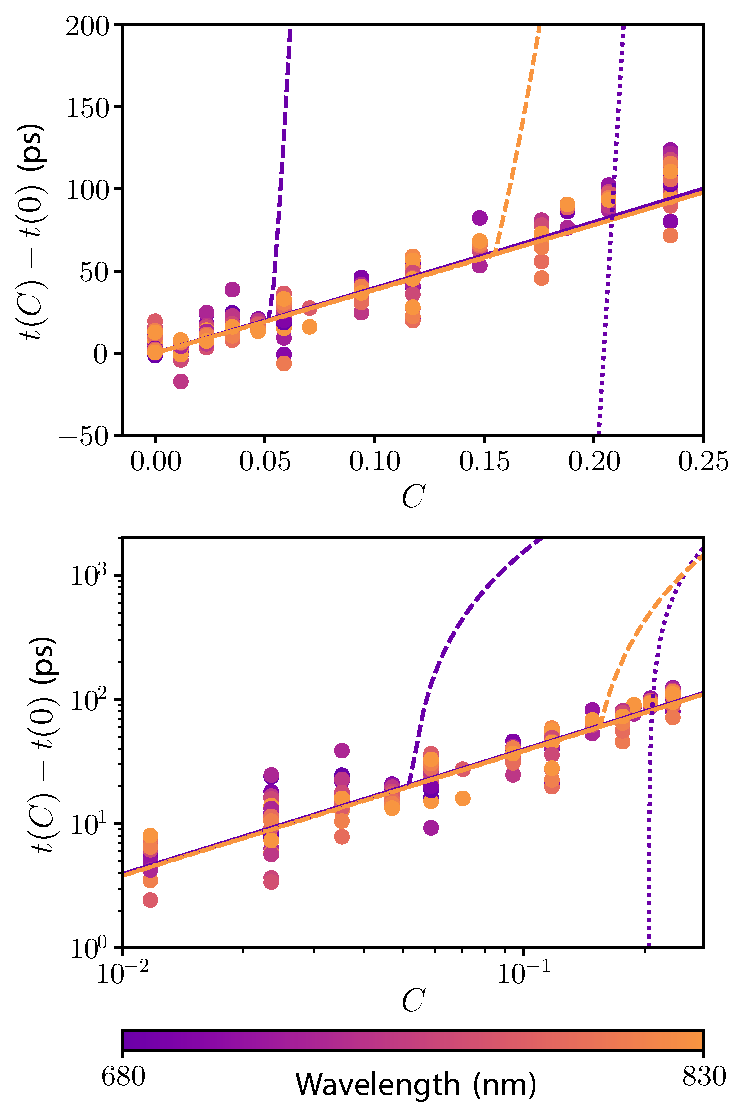
\includegraphics[width=0.8\columnwidth]{Figures/final_predictions_with_data.pdf}
\caption{\label{fig:alldata} EFPT differences measured experimentally, in picoseconds, versus volume concentration $C$. Both plots are the same, with different scales. Solid lines are predicted EFPTs for a photon traveling through an index-averaged medium of silica and water. Experimental values are shown as points, telegraph equation predictions are shown as dashed lines, and the diffusion approximation is shown as dotted lines. Color indicates wavelength from 680 nm (violet) to 830 nm (orange). Predictions were made using $N=5\times10^6$ photons. The orange dotted line does not appear in this figure as the values fail to cross over the measured range.}
\end{center}
\end{figure}

\subsection{Telegraph equation}\label{subsec:teleg} 
The telegraph equation  offers a more accurate model for photon transport, incorporating the ballistic motion of photons. By using asymptotic expansions to approximate a solution to \eqref{eq:RTE} ~\cite{heizler_asymptotic_2012, hoenders_telegraphers_2005, gombosi_telegraph_1993}, accounting for the movement of photons in and out of each direction as opposing ``streams''~\cite{schuster_radiation_1905,durian_two-stream_1996,lemieux_diffusing-light_1998,masoliver_solutions_1992}, or by various other methods of derivation~\cite{goldstein_diffusion_1951,dudko_photon_2005,masoliver_finite-velocity_1996,weiss_first_1984,weiss_applications_2002}, we arrive at a telegraph equation for photon transport~\cite{lemieux_diffusing-light_1998}, which governs the evolution of $\varphi$ as
\begin{align}
     \partial_{r}^{2} \varphi \left(r,t\right)  = &\frac{1}{c^{2}}\partial^{2}_{t} \varphi\left(r,t\right) + \frac{1}{c}\left(2 \mu_{a} + 3 \mu_{s} \right) \partial_{t} \varphi\left(r,t\right) \nonumber \\
    &+ \mu_{a}\left(\mu_{a} + 3 \mu_{s} \right) \varphi. \label{eq:tel}
\end{align}
At short times, \eqref{eq:tel} reduces to the wave equation. At long times and in the limit of $\mu_{a}$ going to zero we recover \eqref{eq:diff}, the standard diffusion approximation, with diffusion coefficient~\cite{lemieux_diffusing-light_1998}
\begin{equation}\label{eq:telD}
    D = \frac{c}{3\mu_{s}}.
\end{equation}

The general solution to this telegraph equation is given by~\cite{goldstein_diffusion_1951,durian_photon_1997}
%
\begin{align}
    \varphi \left(r,t\right) &= \frac{1}{2} e^{-\left(\mu_{a}c + \gamma \right)t} \bigg[\delta \left(c t - r\right) + \delta\left(ct + r\right) \notag\\
    &+\left. \Theta\left(c t - |r|\right) \left(\frac{\gamma}{c}I_{0}\left(\frac{\gamma u}{c}\right) + \frac{\gamma t}{u}I_{1}\left(\frac{\gamma u}{c}\right)\right)\right]
\end{align}
%
where $\delta$ is the Dirac delta function, $\Theta$ is the Heaviside step function, $I_{0}$ and $I_{1}$ are modified Bessel functions of the first kind, $u=\sqrt{c^{2}t^{2}-r^{2}}$ represents the position relative to that of a ballistic photon, and $\gamma = \frac{3}{2} c \mu_{s}$ is a characteristic time scale for scattering events~\cite{goldstein_diffusion_1951,masoliver_solution_1993,masoliver_telegraphers_1994,masoliver_finite-velocity_1996}. We solve this numerically to obtain EFPT predictions.

\section{Results and Discussion}
Figure \ref{fig:alldata} shows $t(C)$, the time of the peak of the EFPT distribution for scatterer volume concentration $C$, for a range of wavelengths and volume concentrations. For each wavelength measured, this time is shown relative to $t(0)$, the time of the peak of the EFPT distribution for pure water recorded at that wavelength. The measured EFPTs show no wavelength dependence and increase linearly with $C$, reaching approximately 100 ps for $C$ = 0.235. The measured EFPT differences are consistent with the extreme photons traveling at the speed of light through a \textit{non-scattering} index-averaged medium at each concentration. 

The predictions of the two models are plotted as dotted lines (diffusion approximation) and dashed lines (telegraph equation) for wavelengths at the extreme ends of our experimental range. These predictions are calculated using $N \simeq 5 \times 10^{6}$. Because the EFPT increases with decreasing $N$~\cite{lawley_distribution_2020}, this upper limit for $N$ provides a lower bound on the predicted values of the peak EFPT. Additionally, the relative difference between the predictions at 680 nm and 830 nm becomes larger as $N$ decreases. The diffusion approximation predicts non-physical results for small concentrations, allowing photons to travel faster than the speed of light for $C$ below approximately 0.21 at 680 nm and at all concentrations for 830 nm.  At higher concentrations, the diffusion approximation predicts increasing EFPT differences  for 680 nm, exceeding 650 ps (680 nm) at $C$ = 0.235. Relatively speaking, the telegraph equation does a better job and predicts a linear relationship for EFPT delay at low concentrations, determined by the speed of light in the index-averaged medium. However, for concentrations beyond approximately 0.05 (680 nm) and 0.15 (830 nm), scattering and absorption cause the EFPT difference to increase rapidly and deviate from the measured values. Maximum predicted delays of 8,000 ps (680 nm) and 900 ps (830 nm) occur at $C$ = 0.235.

\section{Conclusion}
The diffusion and telegraph approximations fail to accurately describe EFPT photons, either violating causality (diffusion) or predicting unrealistically large EFPT differences (diffusion and telegraph). In order to provide accurate predictions, the telegraph equation  would require either unphysically large photon counts of $N \gtrapprox 10^{16}$, far exceeding the laser output to achieve wavelength-independent results, or an anisotropy factor ($\langle \cos {\theta} \rangle \geq 0.4$) that contradicts the isotropic-scattering behavior of Rayleigh scattering. While these models are effective at predicting the behavior of the average photon in scattering media and can be used to infer bulk properties, they fail to describe extreme photons. These results suggest that assumptions made in the underlying random walk approach are incorrect. A model based on random walks which incorporate correlated or even quantum mechanical behavior may produce more accurate predictions and could better describe the underlying physical process. Such a model would unlock the potential for photon EFPT statistics to uncover critical insights about the diffusive environment, with broad applications across many areas of science~\cite{redner_guide_2001,weiss_applications_2002,godec_first_2016,noskowicz_average_1988,grebenkov_molecular_2021,polizzi_mean_2016,barney_first-passage-time_2017,zsurkis_first_2024,lawley_distribution_2020,lawley_slowest_2023,lawley_universal_2020,schuss_redundancy_2019,meerson_mortality_2015,chun_heterogeneous_2023}.

\section{Acknowledgments}
We thank M. Allgaier, J. Hass, D. Allcock, I. Corwin, and R. Parthasarathy for discussions. This work was funded by the W. M. Keck Foundation Science and Engineering grant on ``Extreme Diffusion''.


\chapter{Conclusion}
\acg{first draft}

The random walk model of diffusion has worked very well to describe the average particle, in applications from (one example) to photons (doing something else) to (third example). However, there are many instances in which it fails (cite them) (list them?). Recent mathematical work has proposed alternate models to account for these other cases, from the BC to quantum to whatever. This work measured the extreme value statistics in multiple systems and demonstrated the need for alternate models. First, we measured extreme first passage particle locations in numerical work and found the location to scale as (whatever). Second, we measured extreme first passage times in scattering photons and determined that the location of the peak of the extreme first passage time distribution is controlled by the averaged index of refraction of the scattering medium. Finally, we developed a proof of concept experimental setup to measure extreme first passage times in a system of diffusing silica microspheres. These experiments and simulations shed new light on the extreme value statistics of diffusing systems and how we can measure these statistics in real physical systems to learn about the underlying processes.

We know pretty well how to predict the average particle location in a system undergoing a random walk, especially an independent one. However, we expect particles nearby each other to move in a correlated manner. We can account for correlations for these particles via mathematical models that introduce bias into the random walk step distributions. Average behavior remains the same, but the predictions for the extreme particles differ greatly. Existing literature on extreme particle locations proposes a scaling of (whatever the Lawley papers say). 

We ran simulations of diffusing particles in Chapter \ref{1Drandom}. From these simulations, we measured the location of the furthest particle. For the furthest particles, we found (whatever we found). This is impactful because (reasons). 

Photon transport has been well modelled by the Boltzmann Radiative Transfer Equation, but it's computationally intensive and has yet to be solved analytically (to my knowledge?). As a result, approximations to the equation are made. Assuming a lot of scatterers and minimal absorption, as well as long overall distances, we can approximate with a diffusion or telegraph equation. These work pretty well to predict the average photon behavior, as exhibited by how useful the models are in a wide variety of applications. However, these models rely on the assumption that photon scattering is completely independent and totally elastic. Again, by neglecting correlated movement due to quantum mechanics and/or optical interference, we predict that these models fail the extremes.

In Chapter \ref{photons}, we measured photon extreme first passage times in random media of varying scatterer concentrations. From these measurements, we determined that (what we determined). This is important because (reasons). 

Finally, we have been able to measure average diffusing particles quite well for quite a while. We can predict the average and extreme particle behavior via these random walk models, accounting for correlation via biases. However, we don't know what actually happens unless we make a measurement of the extreme value statistics in a real physical diffusive system.

In Chapter \ref{extras} developed an experimental apparatus to gather first passage times of colloids diffusing through water. This allows us to explore the first passage time statistcs and can reveal (conect to jacogb's fpt paper). 

The work in this dissertation adds new insight to existing literature both on diffusive systems and photon scattering. We measured extreme value statistics in both, and revealed the need for models that account for correlated movement that exists either due to the shared medium or interference effects. We have built an experimental apparatus to measure extreme first passage times in a physical system, and show how much these measurements can reveal about the limits of what we truly know.


%%%APPENDICES
%%BIBILIOGRAPHY
\bibliographystyle{unsrtnat}
\bibliography{thesis}
\end{document}
